%%
%% This is file `sample-sigconf.tex',
%% generated with the docstrip utility.
%%
%% The original source files were:
%%
%% samples.dtx  (with options: `sigconf')
%% 
%% IMPORTANT NOTICE:
%% 
%% For the copyright see the source file.
%% 
%% Any modified versions of this file must be renamed
%% with new filenames distinct from sample-sigconf.tex.
%% 
%% For distribution of the original source see the terms
%% for copying and modification in the file samples.dtx.
%% 
%% This generated file may be distributed as long as the
%% original source files, as listed above, are part of the
%% same distribution. (The sources need not necessarily be
%% in the same archive or directory.)
%%
%% The first command in your LaTeX source must be the \documentclass command.

%\documentclass[sigconf]{acmart}
\documentclass{IEEEtran}
\usepackage[margin=0.75in]{geometry}
\usepackage{makecell}
\usepackage{booktabs}
\usepackage{amsmath}
\usepackage{amsfonts}
\geometry{top=1.2in,bottom=1in}
%\let\Bbbk\relax
%\usepackage{algorithmic}
%\usepackage{algorithm}



\usepackage{graphicx}
\usepackage{subfig}
\usepackage{array}
\usepackage{multicol}
\usepackage{multirow}
\newcolumntype{P}[1]{>{\centering\arraybackslash}p{#1}}
\newcolumntype{M}[1]{>{\centering\arraybackslash}m{#1}}


\newcommand{\blue}[1]{{\color{blue} #1}}
\newcommand{\red}[1]{{\color{red} #1}}


%%
%% \BibTeX command to typeset BibTeX logo in the docs
\AtBeginDocument{%
  \providecommand\BibTeX{{%
    \normalfont B\kern-0.5em{\scshape i\kern-0.25em b}\kern-0.8em\TeX}}}

%% Rights management information.  This information is sent to you
%% when you complete the rights form.  These commands have SAMPLE
%% values in them; it is your responsibility as an author to replace
%% the commands and values with those provided to you when you
%% complete the rights form.
%\setcopyright{acmcopyright}
%\copyrightyear{2018}
%\acmYear{2018}
%\acmDOI{10.1145/1122445.1122456}
%
%%% These commands are for a PROCEEDINGS abstract or paper.
%\acmConference[Woodstock '18]{Woodstock '18: ACM Symposium on Neural
%  Gaze Detection}{June 03--05, 2018}{Woodstock, NY}
%\acmBooktitle{Woodstock '18: ACM Symposium on Neural Gaze Detection,
%  June 03--05, 2018, Woodstock, NY}
%\acmPrice{15.00}
%\acmISBN{978-1-4503-XXXX-X/18/06}


%%
%% Submission ID.
%% Use this when submitting an article to a sponsored event. You'll
%% receive a unique submission ID from the organizers
%% of the event, and this ID should be used as the parameter to this command.
%%\acmSubmissionID{123-A56-BU3}

%%
%% The majority of ACM publications use numbered citations and
%% references.  The command \citestyle{authoryear} switches to the
%% "author year" style.
%%
%% If you are preparing content for an event
%% sponsored by ACM SIGGRAPH, you must use the "author year" style of
%% citations and references.
%% Uncommenting
%% the next command will enable that style.
%%\citestyle{acmauthoryear}

%%
%% end of the preamble, start of the body of the document source.
\begin{document}

%%
%% The "title" command has an optional parameter,
%% allowing the author to define a "short title" to be used in page headers.
\title{DeepER: A Deep Learning based Emergency Resolution Time Prediction System}
\author{ Gissella Bejarano, Adita Kulkarni, Xianzhi Luo, Anand Seetharam, Arti Ramesh
\\ Department of Computer Science, SUNY Binghamton, USA
\\  (gbejara1,  akulka17, xluo22, aseethar, artir)@binghamton.edu
}
%\affiliation{%
%  \institution{Computer Science Department, SUNY Binghamton}
%}
%\email{ (gbejara1,  akulka17, xluo22, aseethar, artir)@binghamton.edu}
%%
%% The "author" command and its associated commands are used to define
%% the authors and their affiliations.
%% Of note is the shared affiliation of the first two authors, and the
%% "authornote" and "authornotemark" commands
%% used to denote shared contribution to the research.
%\author{Ben Trovato}
%\authornote{Both authors contributed equally to this research.}
%\email{trovato@corporation.com}
%\orcid{1234-5678-9012}
%\author{G.K.M. Tobin}
%\authornotemark[1]
%\email{webmaster@marysville-ohio.com}
%\affiliation{%
%  \institution{Institute for Clarity in Documentation}
%  \streetaddress{P.O. Box 1212}
%  \city{Dublin}
%  \state{Ohio}
%  \postcode{43017-6221}
%}
%
%\author{Lars Th{\o}rv{\"a}ld}
%\affiliation{%
%  \institution{The Th{\o}rv{\"a}ld Group}
%  \streetaddress{1 Th{\o}rv{\"a}ld Circle}
%  \city{Hekla}
%  \country{Iceland}}
%\email{larst@affiliation.org}
%
%\author{Valerie B\'eranger}
%\affiliation{%
%  \institution{Inria Paris-Rocquencourt}
%  \city{Rocquencourt}
%  \country{France}
%}
%
%
%%%
%%% By default, the full list of authors will be used in the page
%%% headers. Often, this list is too long, and will overlap
%%% other information printed in the page headers. This command allows
%%% the author to define a more concise list
%%% of authors' names for this purpose.
%\renewcommand{\shortauthors}{Trovato and Tobin, et al.}

%%
%% The code below is generated by the tool at http://dl.acm.org/ccs.cfm.
%% Please copy and paste the code instead of the example below.

%%
%% Keywords. The author(s) should pick words that accurately describe
%% the work being presented. Separate the keywords with commas.
%\keywords{datasets, neural networks, gaze detection, text tagging}

%% A "teaser" image appears between the author and affiliation
%% information and the body of the document, and typically spans the
%% page.
%%
%% This command processes the author and affiliation and title
%% information and builds the first part of the formatted document.
\maketitle


\begin{abstract}
%!TEX root = paper.tex
%Public safety and smooth functioning of cities depend, among other factors, of accurate prediction of response time, especially for emergency incidents.
Accurately predicting resolution time for emergency incidents is crucial for public safety and smooth functioning of cities as it helps in planning resources that will be available for immediate assistance. 
In this paper, we present DeepER, a deep learning based emergency resolution time prediction system that predicts future resolution times based on past data. DeepER is an encoder-decoder based sequence-to-sequence model that uses Recurrent Neural Networks (RNNs) as the neural network architecture. The basic cell in DeepER is a Long Short-Term Memory (LSTM) cell. We perform experiments on the NYC Emergency Response Incidents data provided by NYC Open Data. We compare the performance of the model with ARIMA and Linear Regression using two metrics--- Root Mean Squared Error (RMSE) and Mean Absolute Error (MAE). DeepER achieves an average performance improvement of 3\% and 16\% with respect to RMSE and 10\% and 27\% with respect to MAE over ARIMA and Linear Regression, respectively. %Finally, we provide some insights into the trends in data and preprocessing applied.

%Furthermore, we introduce strong evidence for preprocessing decisions applied to this dataset.

%% RECALCULATE PERCENTAGE WITHOUT UTILITY??

%we discuss some preprocessing criteria applied to a 10\% of outliers and 30\% of missing response time.
\end{abstract}

\section{Introduction}
\label{sec:intro}
%!TEX root = paper.tex

%NYC.gov \cite{nycgov} reports statistics and datasets for a range of domains such as emergency incidents, non-emergency events, crimes, offenses and more. To ensure public safety and smooth functioning of the city, it is important to allocate resources for these types of events efficiently. Particularly, response times for emergency incidents can be reduced and improve the logistics of the office in charge. NYC Open Data portal and the Office of Emergency Management (OEM) provide the Emergency Response Incidents dataset, which is publicly available at \cite{nycopendata} and is updated daily.

A number of emergency incidents (e.g. fire, building collapse, etc.) are reported on a regular basis in cities around the world. It is important that city officials are able to allocate sufficient resources to ensure public safety, smooth functioning of cities and address such incidents in a timely manner.  To  engage the public in coordinating these emergency response services smoothly, governments and city officials have made such data openly available to everyone. By adopting a data-driven approach, cities can efficiently allocate resources,  plan prudently, and thus minimize the loss to human life and property and improve resolution time. 

One of the major challenges in this regard is estimating the resolution time for  emergency events in the future. While emergencies are unpredictable by nature and often happen unexpectedly, it is possible to leverage past resolution time data to predict the resolution time of future events. This is because the nature of the event (e.g., fire), the extent of damage, and the number of personnel and equipment available on site are keys factors that dictate the total time needed to address the issue. For example, if multiple emergencies occur in a colocated manner, then it is likely that the time needed to address each of these issues will be higher than usual because of the division of resources. Therefore, if a data-driven analysis suggests that resolution time for future events will be higher than a desired value for a particular incident type, then this analysis can provide insights into budget spending, personnel hiring, and resource allocation.


Hence, in this paper, we design \textbf{DeepER}, a deep learning based emergency resolution time prediction system that predicts the future resolution time of incidents based on historical data. We consider three important emergency incident types, namely, \textit{Fire}, \textit{Law} and \textit{Structural}. We model emergency resolution time prediction as a time series prediction problem. At the core of DeepER there is a sequence-to-sequence encoder-decoder neural network architecture. Both the encoder and the decoder in DeepER are Recurrent Neural Networks (RNNs) and the basic cell is an LSTM cell. The encoder receives the previous resolution times as input and encodes them into a hidden context vector. This hidden vector is given as an input to the decoder, which generates future resolution times.

To evaluate the performance of DeepER, we perform extensive experiments on the publicly available NYC Emergency Response Incidents dataset \cite{nycopendata}. We use the data for a period of approximately eight years for the three incident types. This dataset is challenging from the perspective of time series analysis and prediction because emergency events by nature occur at random times (i.e., lack periodicity), have limited correlation to each other and may not follow seasonal trends. Because of this reason, we design DeepER as a sequence-to-sequence model so that it can unearth  the dependencies among the data points in the sequence even though the time period between two consecutive events in the sequence is varying. DeepER leverages these hidden patterns in data to make superior predictions.

%, where each incident type has multiple sub types. 
%Different sets of fixed number of consecutive events do not occur in a fixed-time period. %In other words, the number of events for each incident type differ within days, months and years. 
%The incidents for which response times are recorded do not occur in a fixed time interval. This non-equidistant characteristic of the dataset makes the prediction task challenging, specially in the search of dynamic-length patterns. 

We compare the performance of DeepER with two widely used baselines--- Linear Regression and Auto Regressive Integrated Moving Average (ARIMA). We use two metrics to evaluate the models--- Root Mean Squared Error (RMSE) and Mean Absolute Error (MAE). DeepER achieves an average performance improvement of 3\% and 16\% with respect to RMSE and 10\% and 27\% with respect to MAE  over ARIMA and Linear Regression, respectively. Our results demonstrate that DeepER is a practically viable system that provides superior prediction performance and can be used to aid city planning and management. We conclude the paper with a discussion of some of the insights we obtain while conducting this investigation.

The rest of the paper is organized as follows. In Section \ref{sec:related}, we present related work. We present  the dataset and discuss the problem investigated in this paper in Section \ref{sec:data}. We then describe the DeepER system in Section \ref{sec:model} and the implementation details in Section \ref{sec:implementation}. We present experimental results in Section \ref{sec:results} and discuss some of our insights from this work in Section \ref{Data:Discussion}.

%Our main contributions are as follows:
%
%\begin{itemize}
%\item We propose \textit{DeepER}, a deep learning based emergency response prediction system, that uses past data to predict future response times. \textit{DeepER} is an encoder-decoder based system which consists of two components --- an encoder which is a Long Short Term Me
%\end{itemize}


\begin{figure*}[!ht]
    \centering
  \subfloat[Fire]{%
       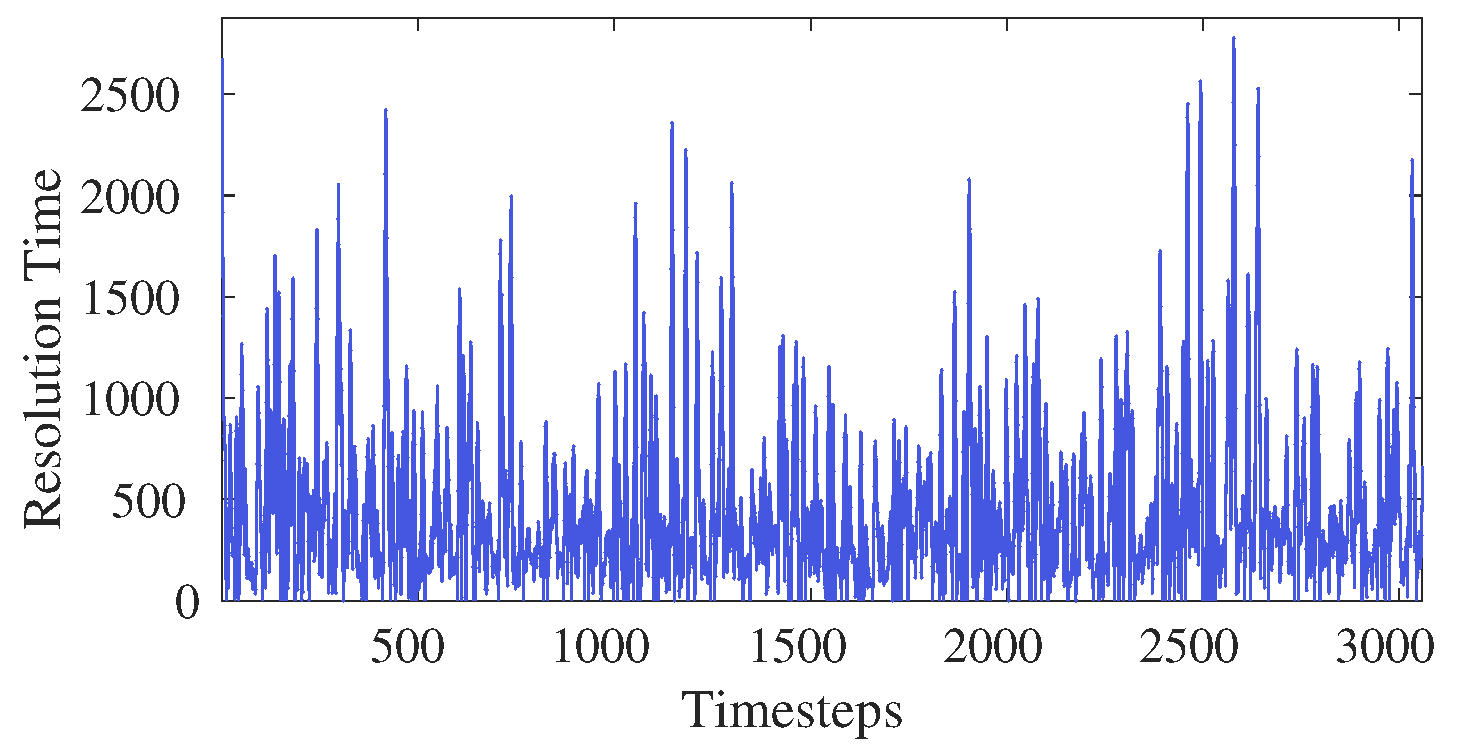
\includegraphics[scale=0.23]{Figures/Data/FullData/Fir}
       \label{1a}}
  \subfloat[Law]{%
       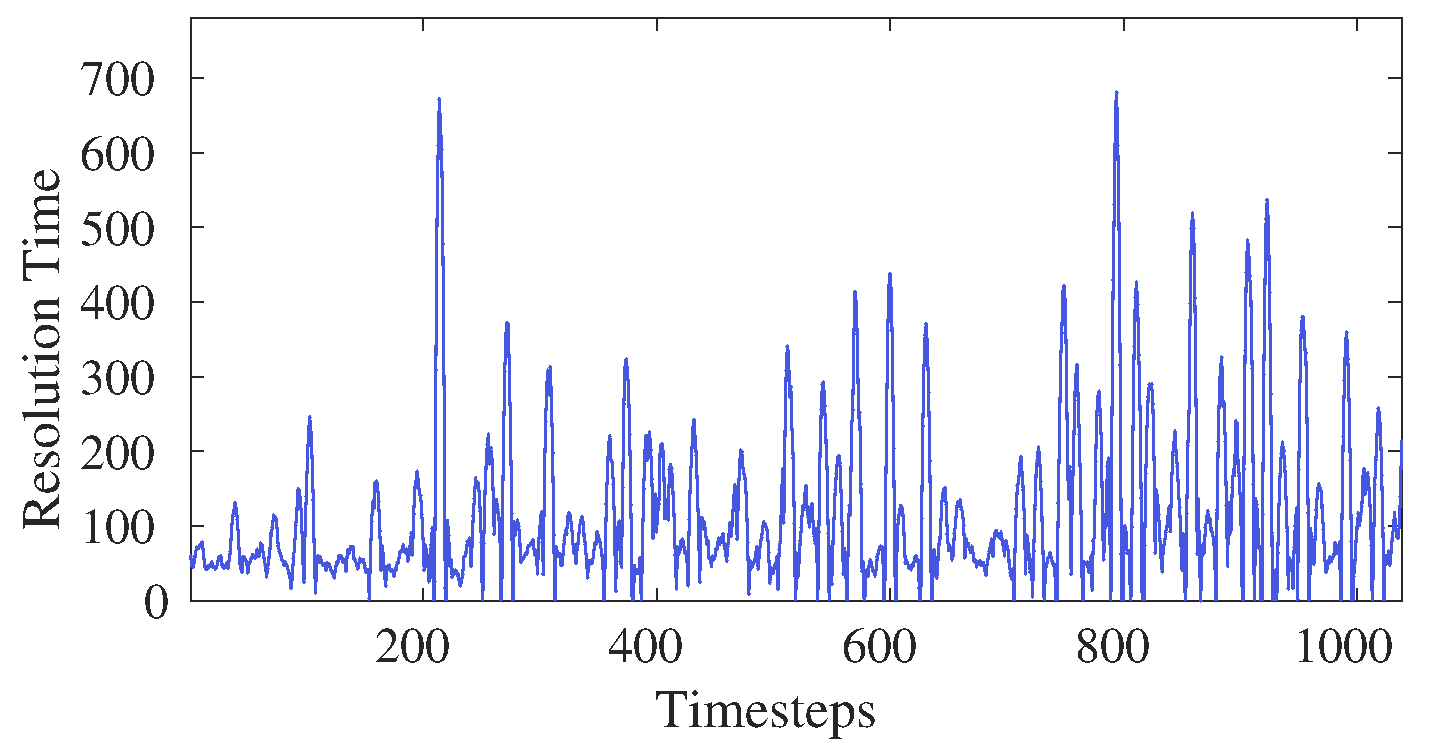
\includegraphics[scale=0.23]{Figures/Data/FullData/Law}
       \label{1b}}
  \subfloat[Structural]{%
       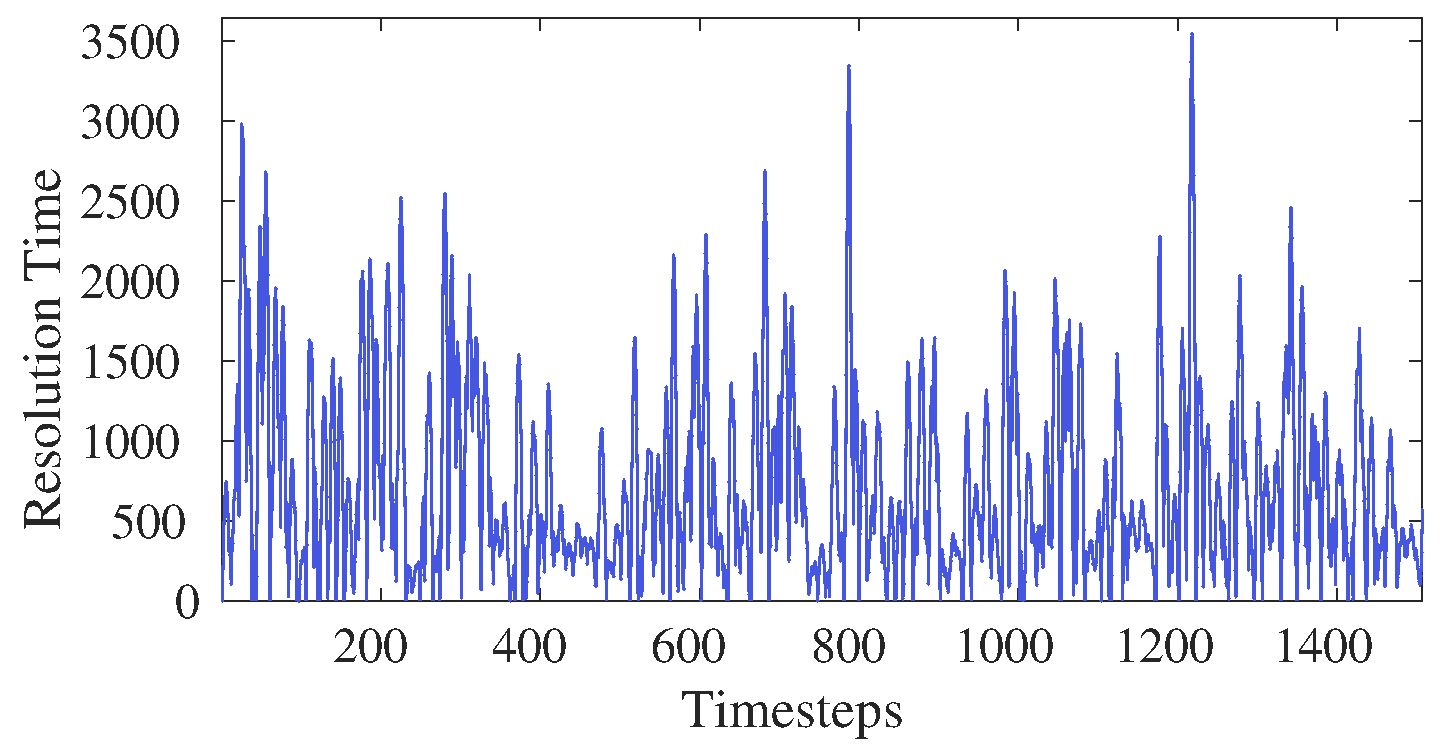
\includegraphics[scale=0.23]{Figures/Data/FullData/Str}
       \label{1c}}
  %\subfloat[Utility]{%
  %     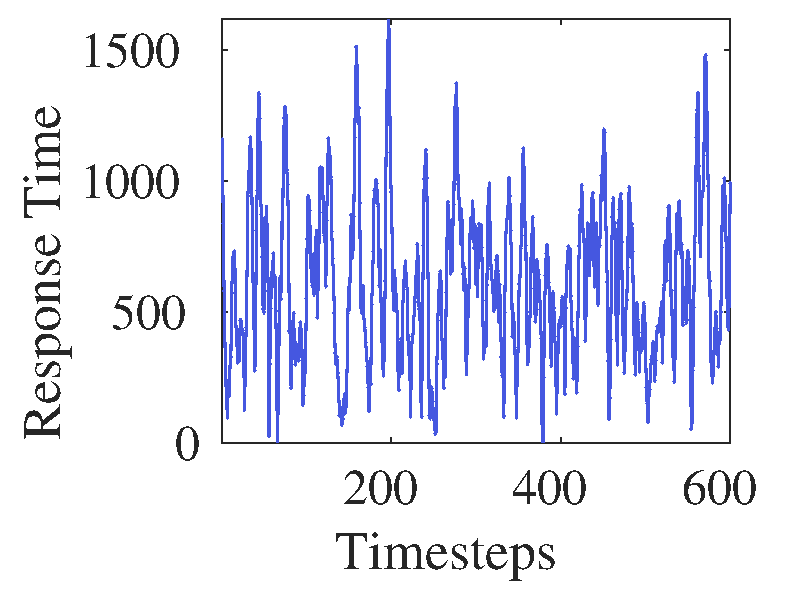
\includegraphics[scale=0.31]{Figures/Data/Uti}
  %     \label{1d}}
	\caption{Trends in datasets}
  \label{fig:trend} 
  \vspace{-3mm}
\end{figure*}

\begin{figure*}[!ht]
    \centering
  \subfloat[Fire]{%
       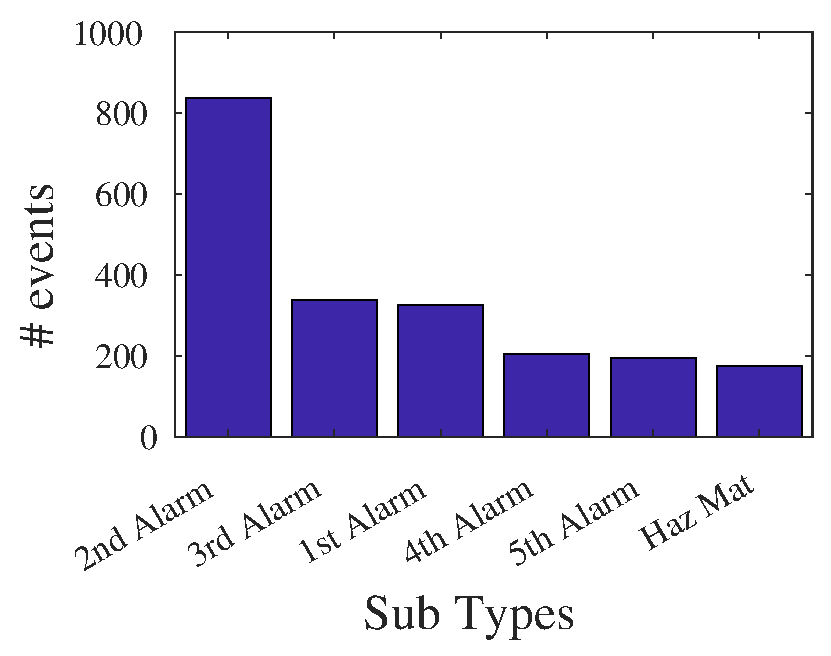
\includegraphics[scale=0.35]{Figures/Data/SubType/fire}
       \label{2a}}
       %\vspace{5mm}
  \subfloat[Law]{%
       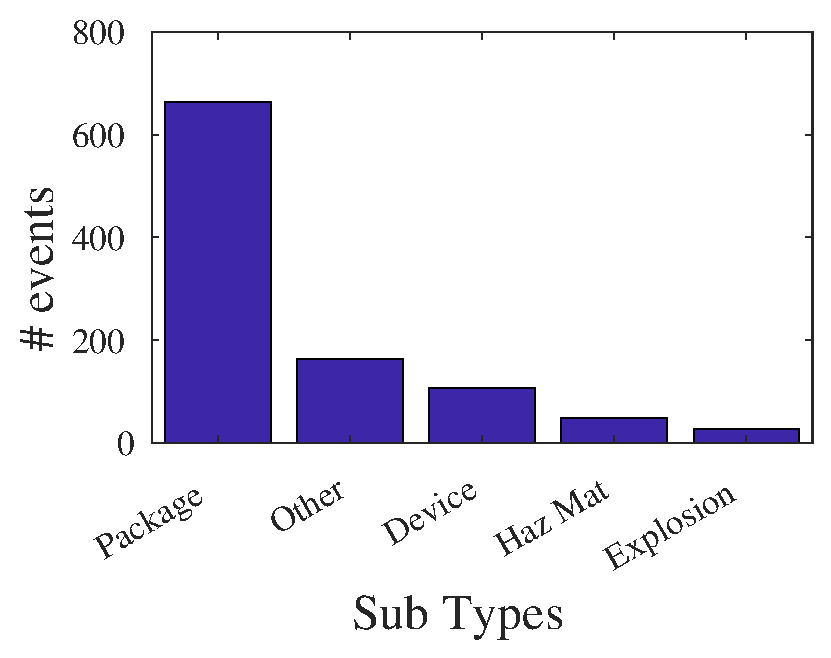
\includegraphics[scale=0.35]{Figures/Data/SubType/law}
       \label{2b}}
       %\vspace{5mm}
  \subfloat[Structural]{%
       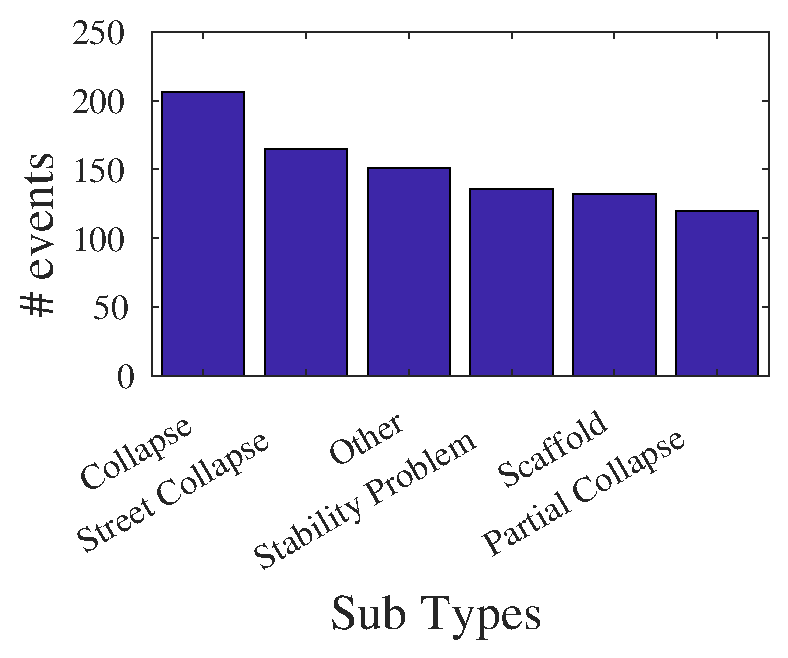
\includegraphics[scale=0.35]{Figures/Data/SubType/structural}
       \label{2c}}
  %\subfloat[Utility]{%
  %     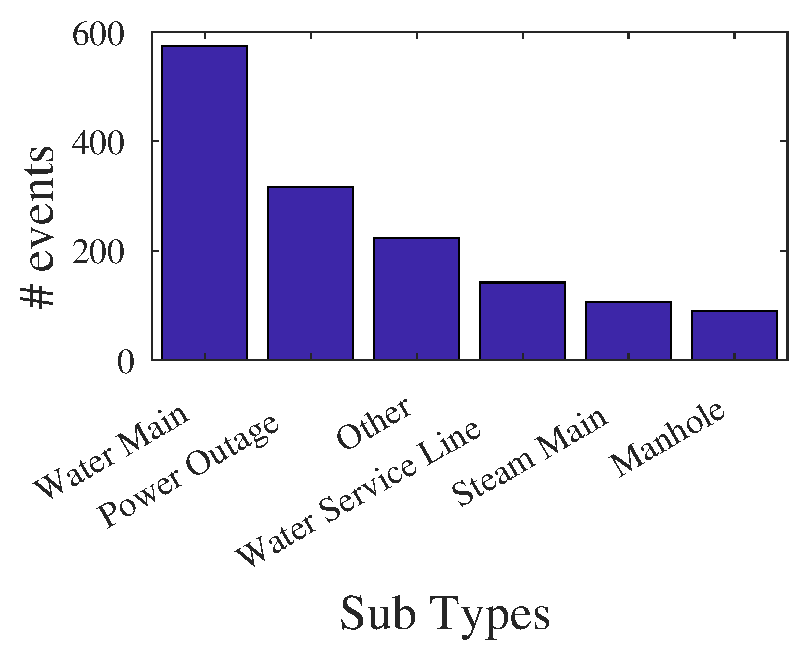
\includegraphics[scale=0.31]{Figures/Data/SubType/utility}
  %     \label{2d}}
	\caption{Incident Types}
  \label{fig:subtype} 
  \vspace{-3mm}
\end{figure*}


\section{Related Work}
\label{sec:related}
%!TEX root = paper.tex

With the growth and development of smart cities and cyber-physical systems, a variety of machine learning approaches have been adopted to address different problems in these domains \cite{Fox, 6894591, AROMA, Guan, AAAI1816607,Varamin}. In this section, we first present work related to assisting the operations of emergency and non-emergency  services and then discuss  prior research related to smart cities.

In the recent years, a number of research papers have adopted data-driven approaches to aid the functioning of emergency and non-emergency  services in cities. For example, DeFazio et al. use Gaussian Conditional Random Fields (GCRFs)  to predict  response times of non-emergency  311 calls in NYC  \cite{DeFazio}.  The authors in \cite{ChohlasWood2015Mining9C}  adopt  a rolling forecast model to predict the number of emergency calls  based on the number of 911 calls in NYC. Similarly, the authors analyze NYC non-emergency call requests and present a Random Forest model to predict the number of requests  \cite{Zha2014ProfilingAP}.  

In \cite{Zhao}, authors analyze the intra-region temporal correlation and the inter-region spatial correlation of data collected from NYC and build a framework to predict the number of crimes for certain regions. Similarly, the authors propose a neural network based continuous conditional random field model  for fine-grained crime prediction in Chicago and NYC \cite{yi2019neural}.  The potential of deep learning models for a variety of time series prediction tasks has also been explored recently.  For example, deep learning models have been adopted for emergency event prediction in \cite{CORTEZ2018315}. Similarly, the authors use LSTM based deep models for gas consumption and occupancy detection using WiFi  beacons  in  \cite{Pathak} and \cite{Qolomany}, respectively.  Recurrent Neural Network (RNN) based encoder-decoder models similar to the one designed in this paper have also been used for prediction problems in a variety of different domains.  For example, such models have been used for water consumption,  gym center occupancy, wireless channel quality and air pollution prediction  \cite{SWaP, DeepFit, 8884240, reddy2018deep}. 


 In contrast to existing work, we design DeepER, a deep learning model  to predict the resolution time of emergency services and validate the efficacy of the model using the emergency incidents response data from NYC collected over a period of approximately eight years.

%A benchmark in a new dataset is established in \cite{WANG2020105120}  using a variational auto-encoder and context-based sequence generative neural network. 
 

%%% missing: WANG2020105120 crime spatio-temporal
%%% Widiasari: flood prediction

%, ChohlasWood2015Mining9C, forecasting, regression
% 8421325, % does not apply, sentiment analysis for improving response time
% falcon2018predicting, % floor level 911 prediction
% Campos, %virtualreality
% MUHAMMAD201830, % \textit{Fire} prediction image based
% Zha2014ProfilingAP, % profiling as in describing severa statistics of spatio-temporal and predicting NER calls with random forest
% yi2019neural % CRF CNN crime prediction temporal-spatial, confirm
% Zhao % temporal-spatial crime prediction using ADMM \cite{Boyd}
% BANDARA2020112896 % time series clustering

% Dong2020 urban flood spatio-temporal probability prediction.  The first applies a hybrid model combining FastGRNN \cite{Kusupati} and FCN \cite{karim2017lstm} to predicts the probability of having an urban flood given spatio-temporal variables in a county in Houston.

%In this section, we discuss the existing literature and how it differs from DeepER.

% \cite{w11091808} implements an LSTM that incorporates not only past data but future weather forecast variables to predict hourly weather runoff flow. 


% Widsiasari: use of an LSTM model to predict water level but seems of poor quality
% \cite{Bande} flood prediction with neural network only, seems one time step. I though on including it in the first part, continous value

%All the existing works presented focus in either predicting variables or number of events in a fixed-time period or predicts only the one next time step. Furthermore, most of the deep learning approaches  implement an RNN (or LSTM) whose input and output are part of a same deep learning component. We present DeepER, a system that efficiently predicts future response times for emergency incidents using an encoder-decoder approach. As mentioned before, this consists of two components, an LSTM that works as an encoder, and receives as input the previous time steps, and an RNN that decodes the past data and output a multi-step prediction. We formalize this task in the next sections. Finally, all previous work focus on equidistant time series while we work with response times that represent consecutive non-equidistant time steps.

\section{Data}
\label{sec:data}
%!TEX root = paper.tex

% Brought from introduction
%NYC.gov \cite{nycgov} reports statistics and datasets for a range of domains such as emergency incidents, non-emergency events, crimes, offenses and more. NYC Open Data portal and the Office of Emergency Management (OEM) provide the Emergency Response Incidents dataset, which is publicly available at \cite{nycopendata} and is updated daily.

We use the emergency response incidents data from NYC Open Data provided by the Office of Emergency Management \cite{nycopendata}. We use around 8 years of data starting May 2011 to December 2019. The dataset consists of 13 incident types with 7 attributes each. We use three attributes from the dataset --- Incident type, Creation date, and Close date. In this study, we focus on three of the most important and frequent emergency types --- \textit{Fire}, \textit{Law}, and \textit{Structural}. We calculate the {\it resolution time} for each incident by subtracting the creation date from the close date and converting it to minutes. %and Utility. 
Figure \ref{fig:trend} shows the resolution times for these incidents. We observe that the time required to resolve events related to \textit{Law} is the least followed by %utility, 
\textit{Fire} and \textit{Structural}, respectively. We also observe from Figure \ref{fig:trend} that there is significant variation in resolution time for events belonging to the same incident type.

%In this section, we explain with more detail the reasoning behind our preprocessing criteria and show how some statistics varies according to this, Table \ref{table:stats} shows the response time statistics (mean, standard deviation) for the four incident types before and after the preprocessing steps. 

{Additionally, we observe from the data that each of these three incident types have multiple subtypes, which we extract from the type description.  \textit{Fire}, \textit{Law}, and \textit{Structural} have 52, 29, and 73  subtypes, respectively.  Figure \ref{fig:subtype} shows the  incident subtypes that contribute the most events for each of the most general incident types. We observe that \textit{2nd alarm}, \textit{Suspicious Package (denoted as Package)}, and \textit{Collapse} %and \textit{Water Main} 
are the subtypes that account for the highest number of events in \textit{Fire}, \textit{Law}, and \textit{Structural}%and Utility 
, respectively.





\subsection{Preprocessing}
\label{Data:Preprocessing}

As is the case with most data-driven solutions to real-world problems, the first step involves pre-processing the data to identify missing values and outliers.  We observe that the dataset contains non-trivial number of missing values for events. A missing value is encountered when an event does not have  a valid close date. In the entire dataset, we observe that  \textit{Fire}, \textit{Law}, and  \textit{Structural} have 32\%, 12\%, and 23\%  missing values, respectively.  For each incident type, we replace these missing points by sampling from the actual distribution of the remaining points. To determine the actual distribution for each incident type, we fit the data to more than 80 different distributions. We perform  the Kolmogorov-Smirnov  goodness of fit test (KS test) and use the \textit{p-value} of the KS test to pick the best distribution for the dataset under consideration. 


%We select the distribution with the maximum $p\_value$. If we happen to get some negative values or outliers again, we replace them with zero and quantile 90 of the incident type respectively. We support and explain with more details all these preprocessing decisions in section \ref{Data:Discussion}.

%and utility has 31\% 


We also observe that the dataset contains some outliers---values that are significantly different from the rest of the data points.  By studying the values, we believe that such values might be the result of manually closing some unfinished entries at a later date. For example, we observe some extreme outliers in the dataset (greater than 100,000 minutes). We identify outliers as those points whose resolution time is greater than the quantile 90 of that incident type. For  \textit{Fire}, \textit{Law}, and  \textit{Structural}, we observe that there are 7\%, 9\%, and 8\% outliers, respectively.  Figure \ref{fig:before_after} shows the distribution of  the three different incident types before and after preprocessing.  We observe from the figure that the raw dataset has a large number of outliers.  We once again replace these outliers by sampling from the  distribution of the valid data points. In comparison  to Figure \ref{fig:beforeprocess}, we observe that Figure \ref{fig:afterprocess} presents a significantly refined distribution.


\begin{figure}[!ht]
    \centering
  \subfloat[Before preprocessing]{%
       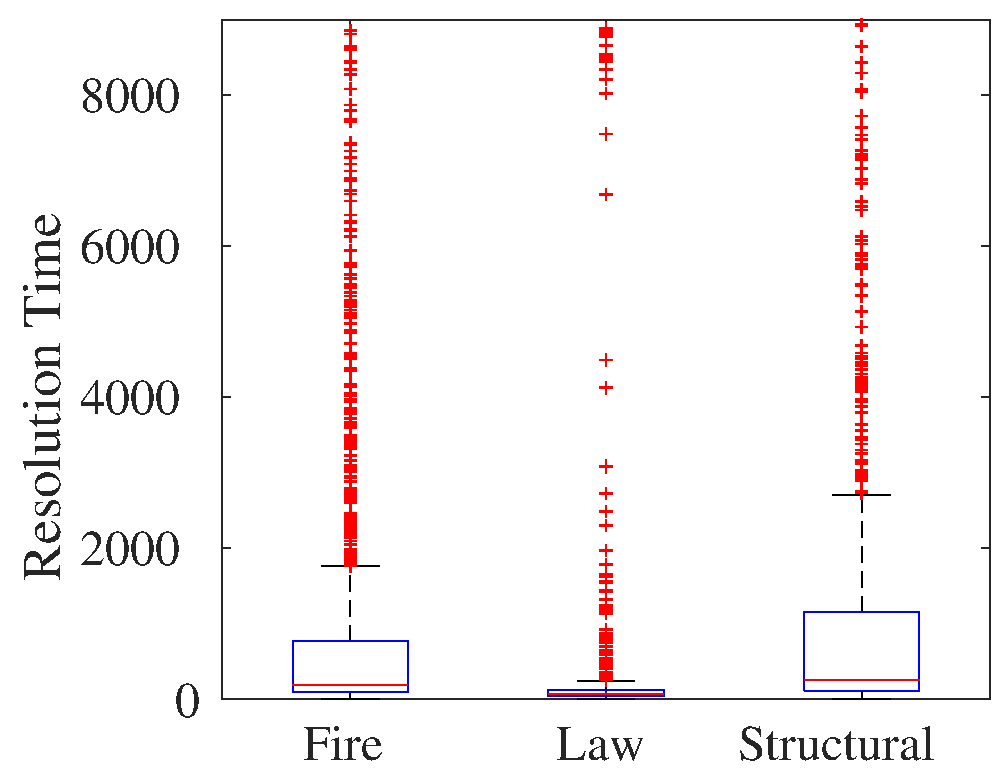
\includegraphics[scale=0.25]{Figures/Data/Boxplot/All_Incidents_before}
       \label{fig:beforeprocess}}
%  \vspace{1mm}
  \subfloat[After preprocessing]{
       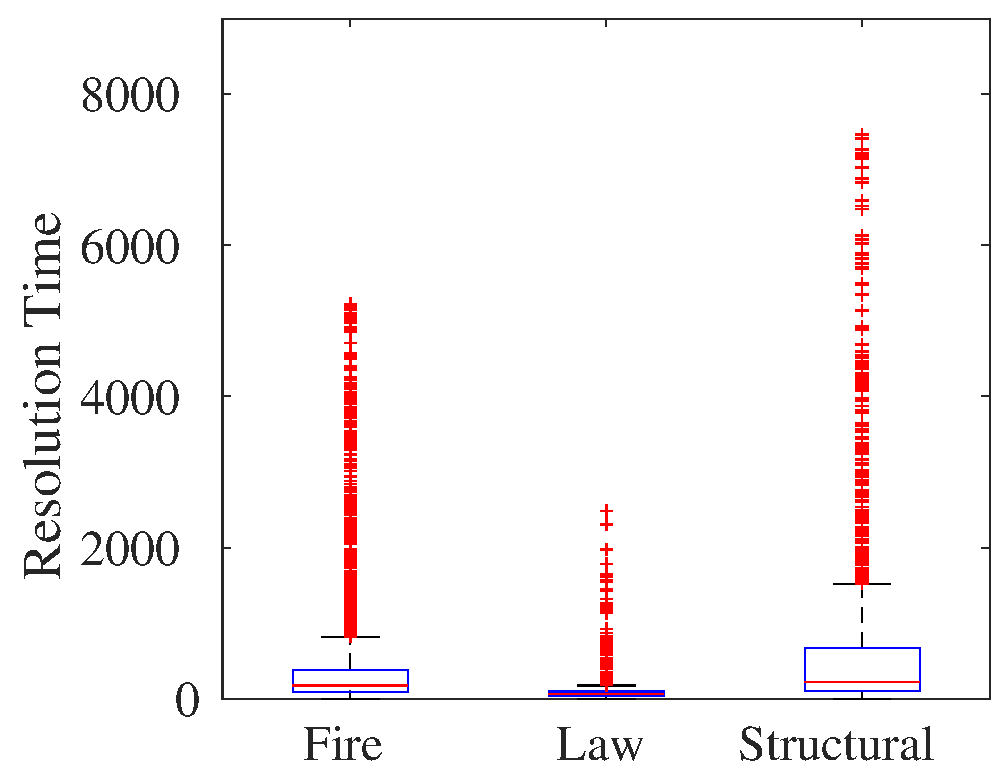
\includegraphics[scale=0.25]{Figures/Data/Boxplot/All_Incidents_after}
       \label{fig:afterprocess}}
	\caption{Datasets before and after preprocessing}
  \label{fig:before_after} 
  \vspace{-1mm}
\end{figure}


We observe some other interesting issues in the dataset. We observe that for {\it Fire} and {\it Structural} most of outliers are located in the first  few years of the dataset. In comparison, most of the missing points are located during the last few years.  Additionally, for {\it Fire} and {\it Structural} we observe larger resolution times during the initial years than the last few years. However, the opposite is true for \textit{Law},  where the resolution times during the initial years is lower than the resolution times in the later years. 


%We use two approaches to perform this replacement --- 1) Sample randomly from the valid points of the training set, and 2) Fit a distribution to each incident type and sample continuous values from these distributions using training set. 


 %\blue{As both these approaches show similar results, in the rest of the paper, we only report results using the second replacement approach.}





%On the other hand, before preprocessing, the values of outliers are very large although , for visualization reasons.
%the input and prediction lengths $m$ and $k$. 








%We aim to design a model that is flexible enough to model any sequence of incidents time frame and can recognize patterns independent of the frame duration. For this time series problem, instances of consecutive fixed number of incidents belong to different time frames. 


%%%%%%%%%%%%%%%%%%% CONFIRM: table values PREV without outliers





%\begin{figure}[!ht]
%    \centering
%  \subfloat[Fire]{%
%       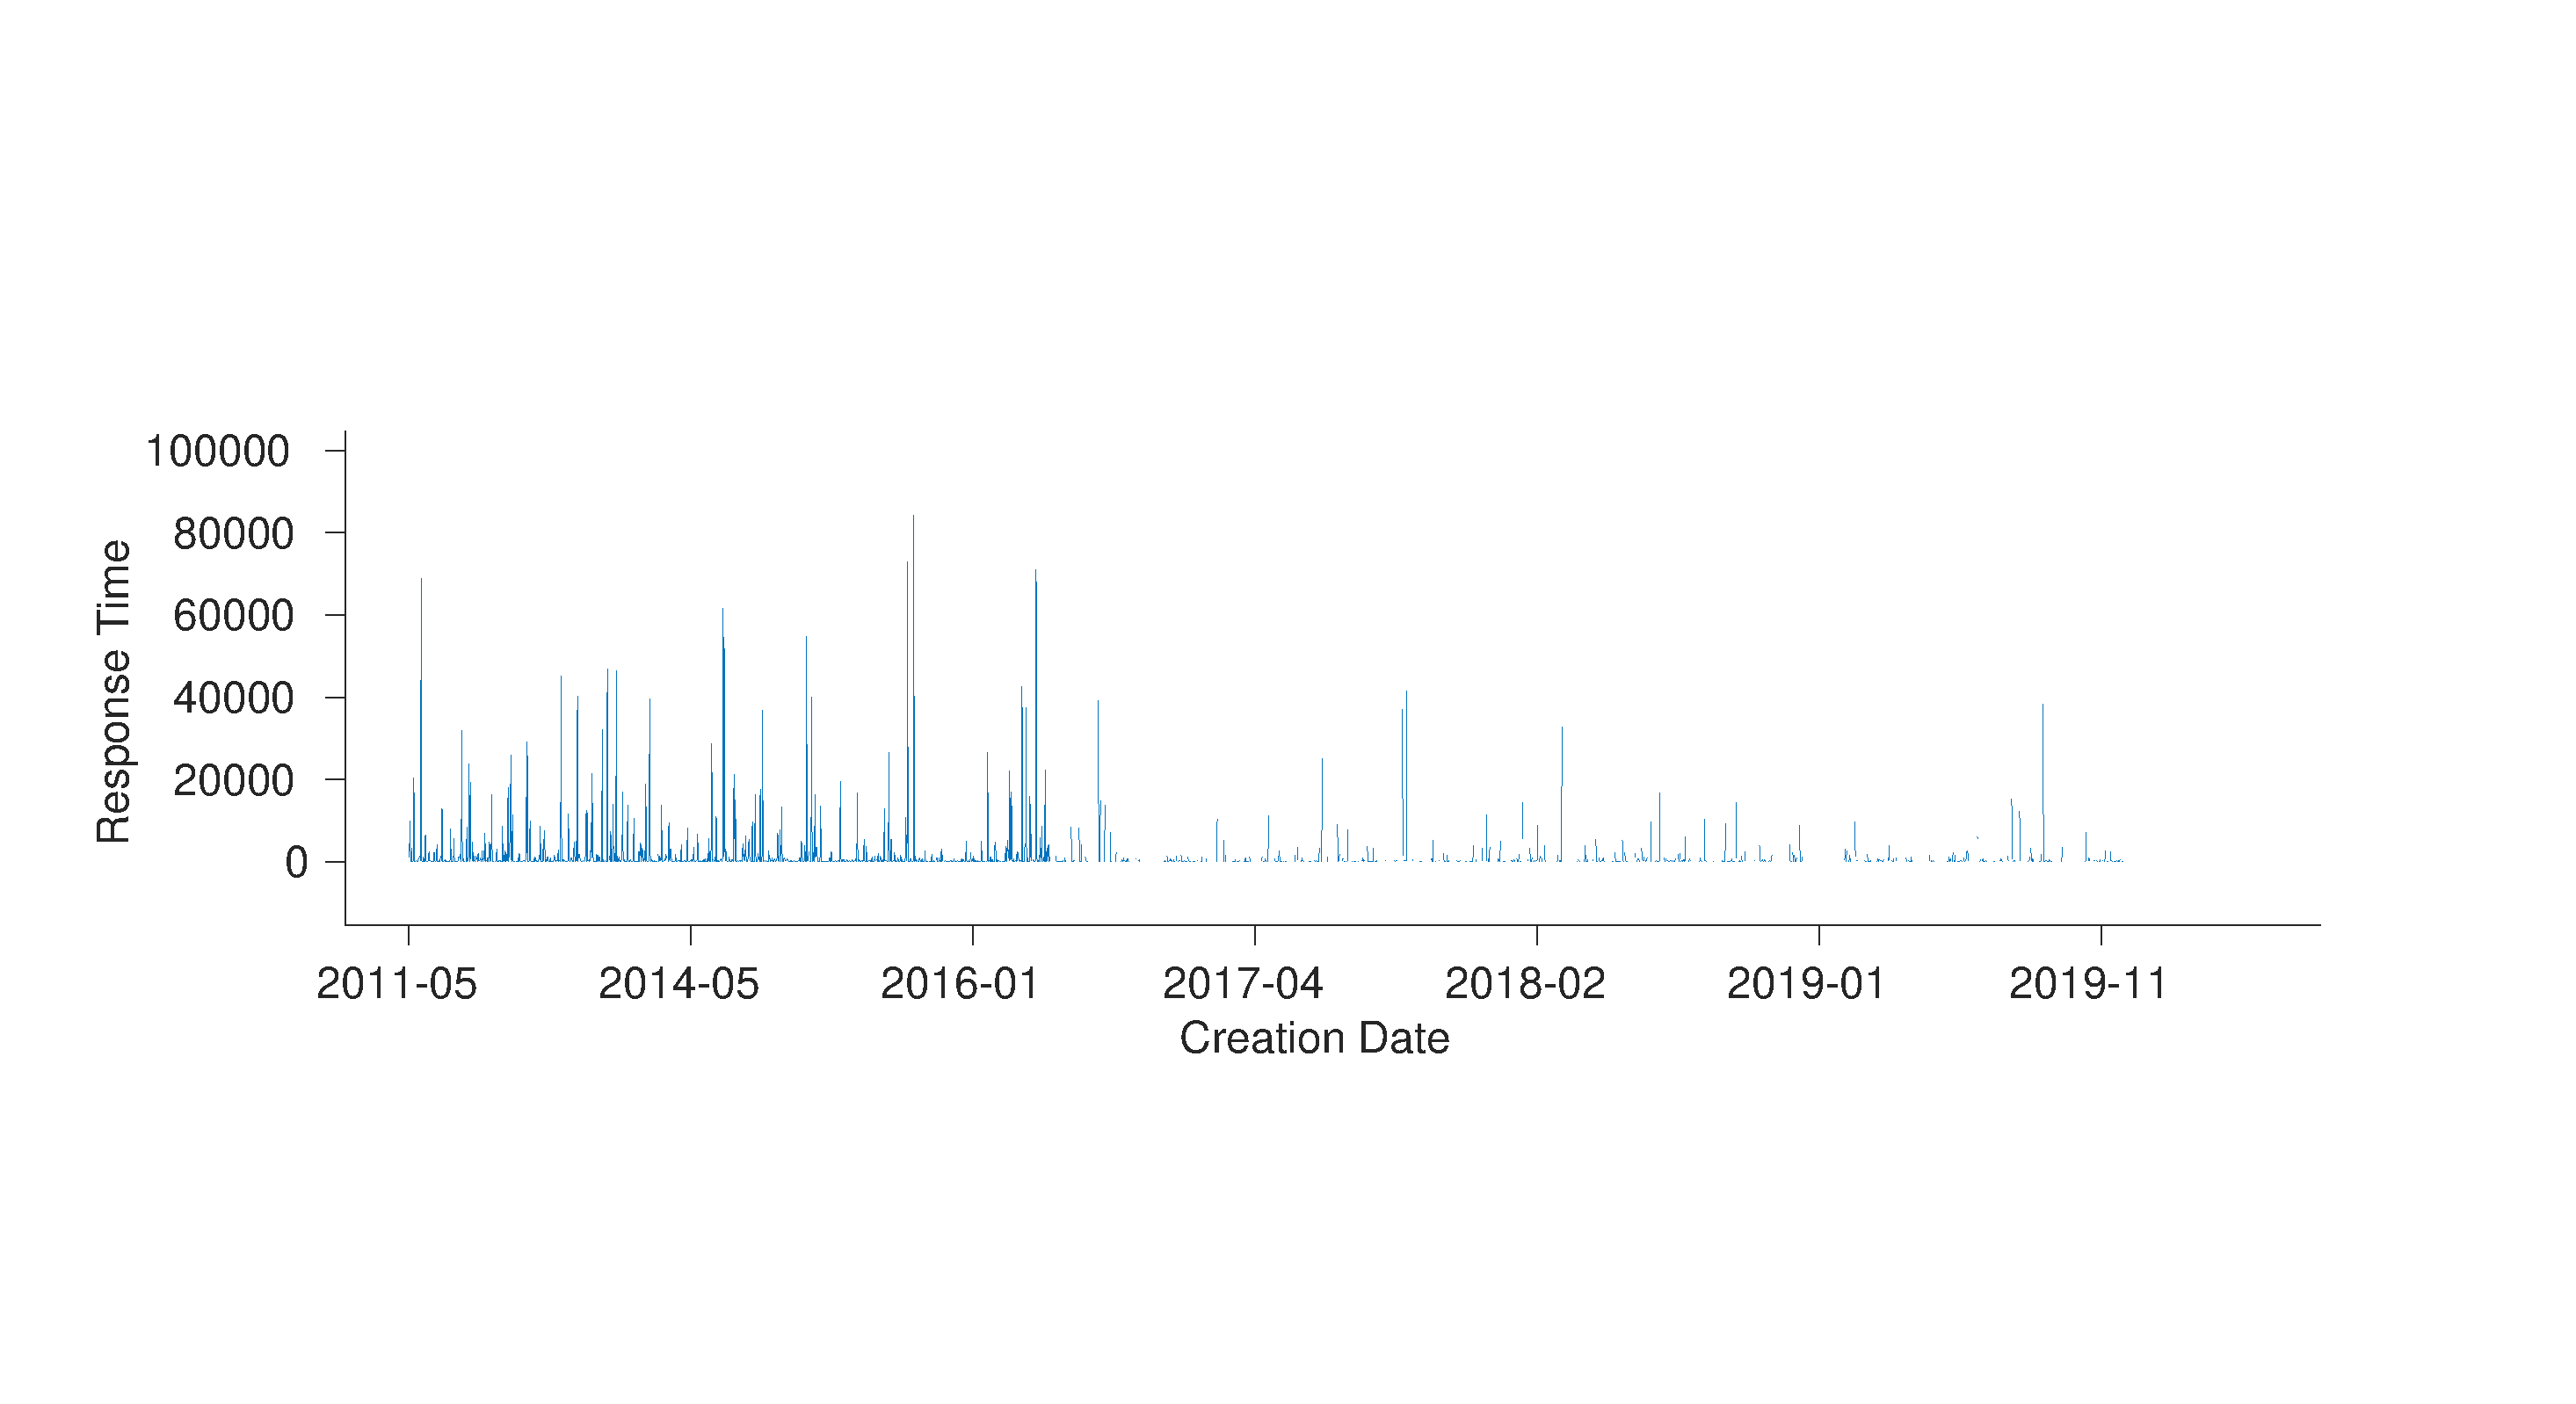
\includegraphics[trim=40 150 150 200,clip,width=1.0\linewidth]{Figures/replacementBinary/plotOutMissFire_mat}%[trim=130 250 150 250,clip,width=1.0\linewidth]{Figures/replacementBinary/plotOutMissFire_mat}
%       \label{4a}}
%  \vspace{1mm}
%  \subfloat[Law]{%
%       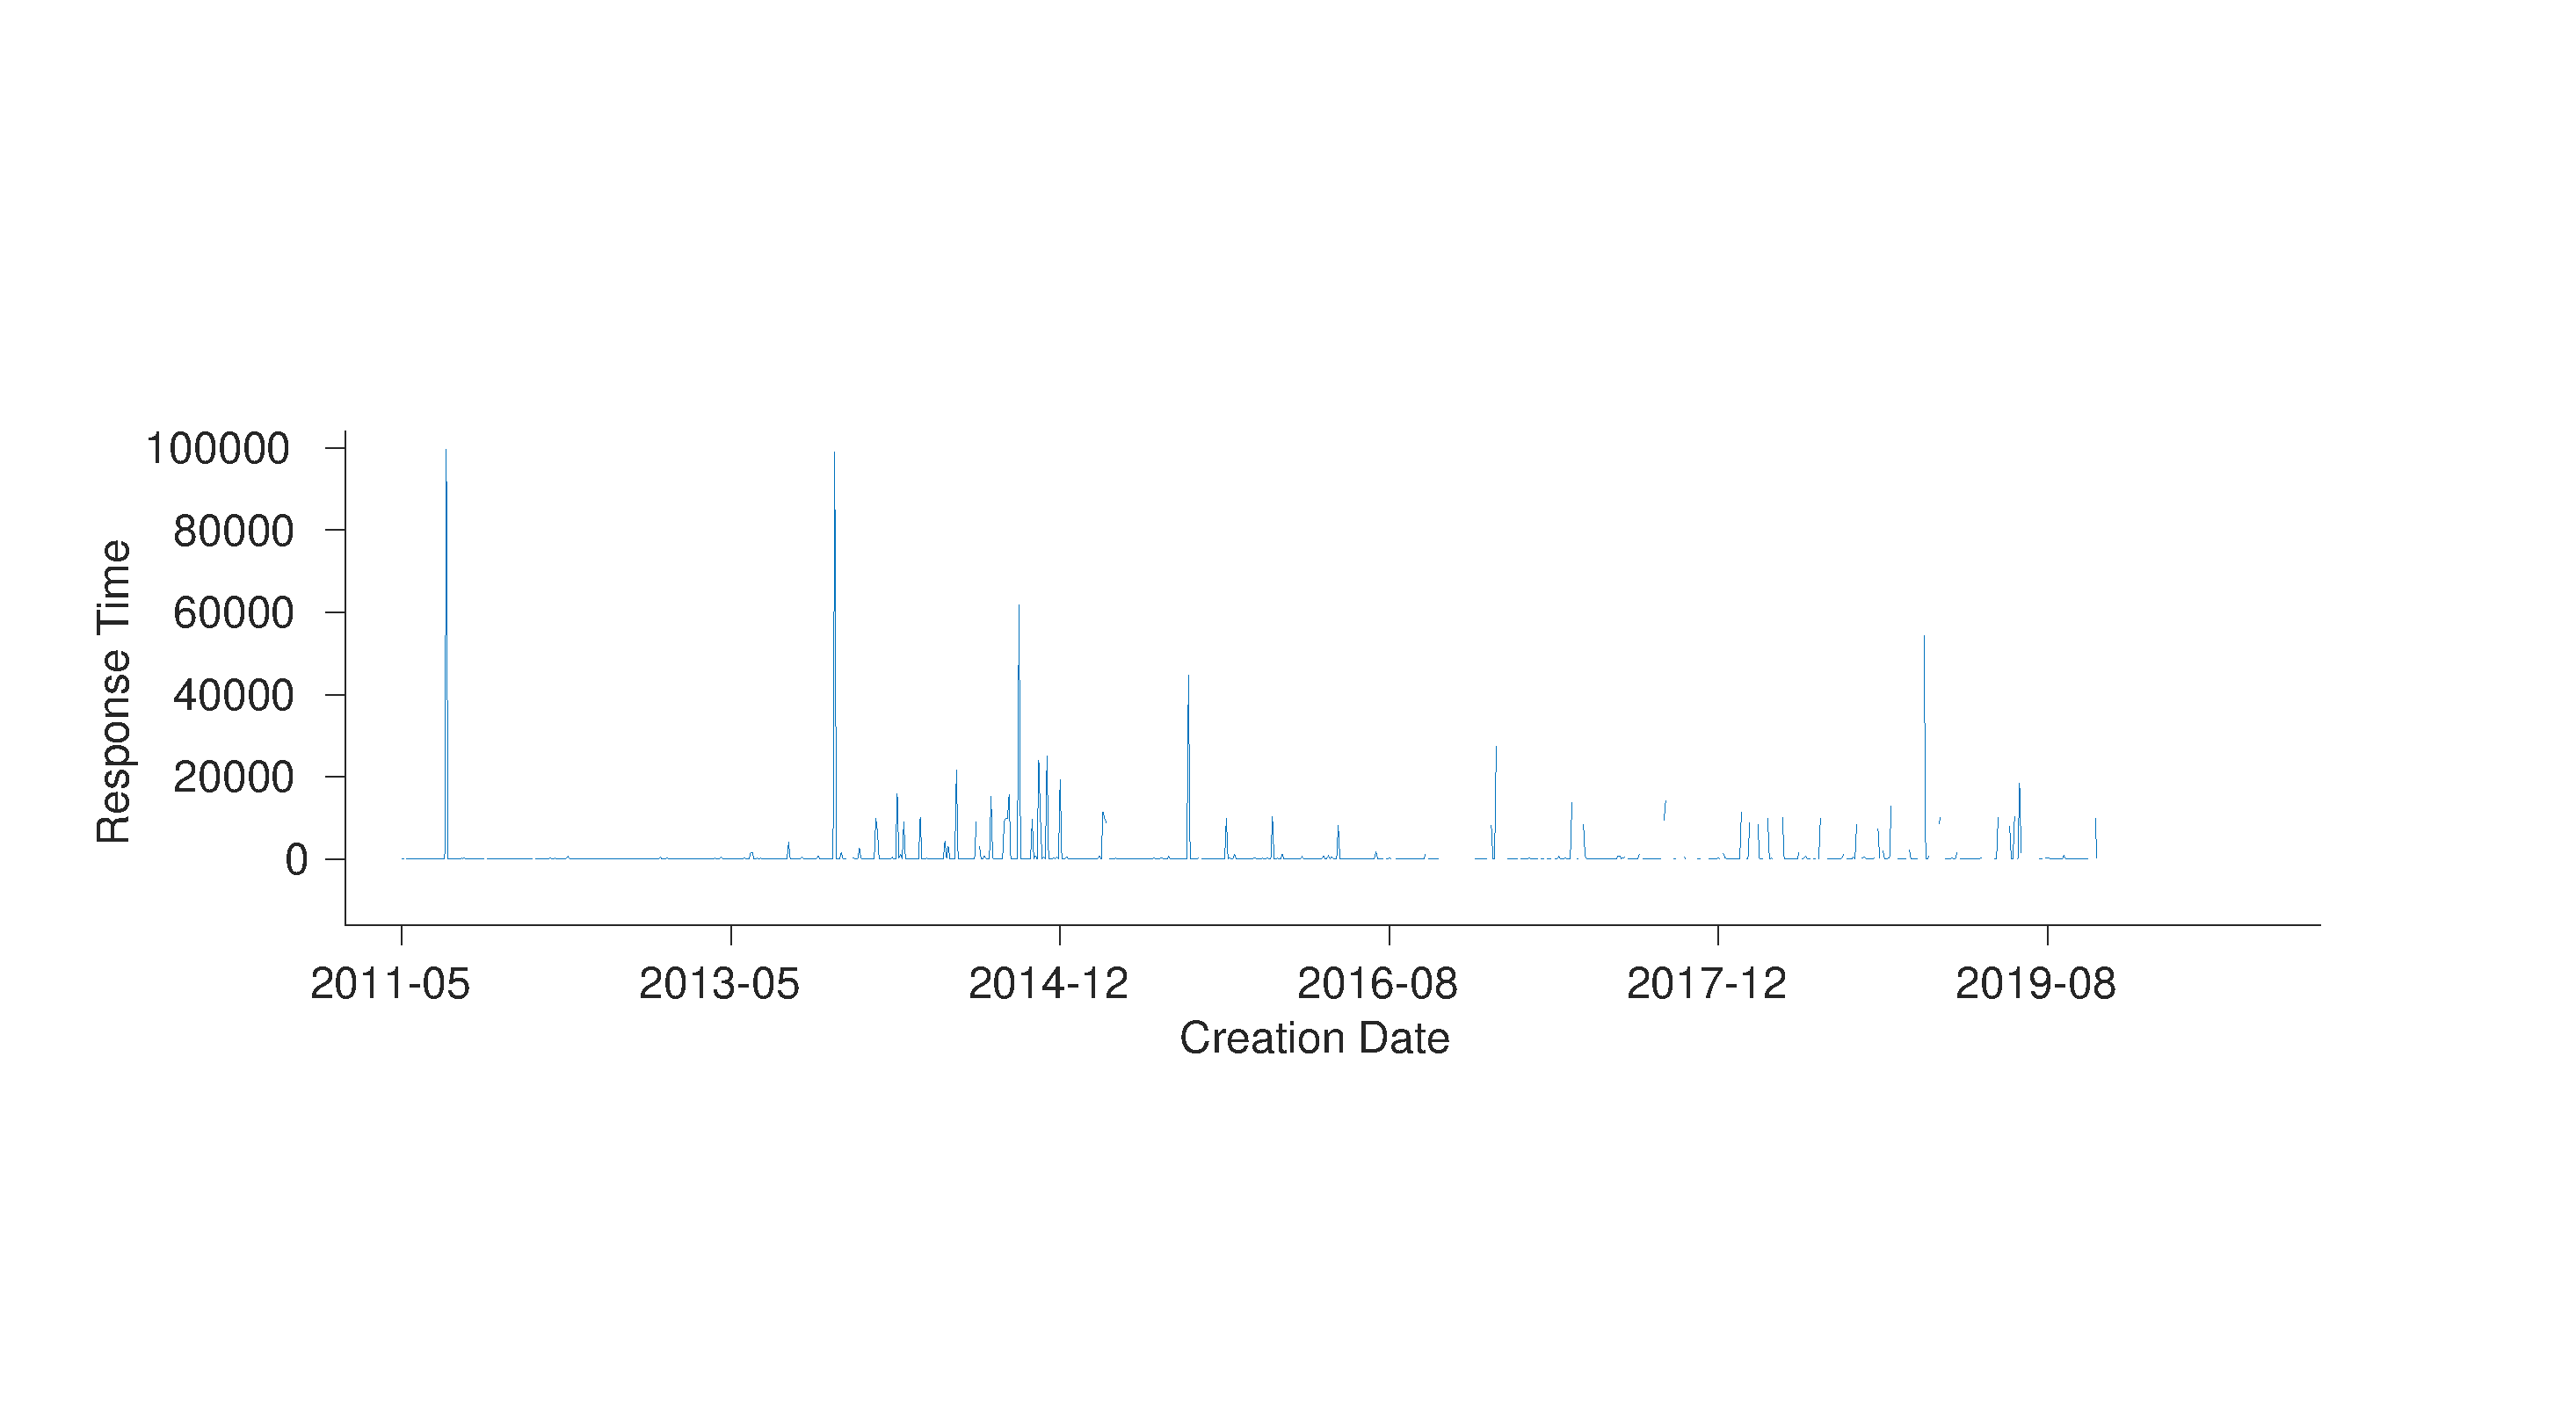
\includegraphics[trim=40 150 150 200,clip,width=1.0\linewidth]{Figures/replacementBinary/plotOutMissLaw_mat}
%       \label{4b}}
%  \vspace{1mm}
%  \subfloat[Structural]{%
%       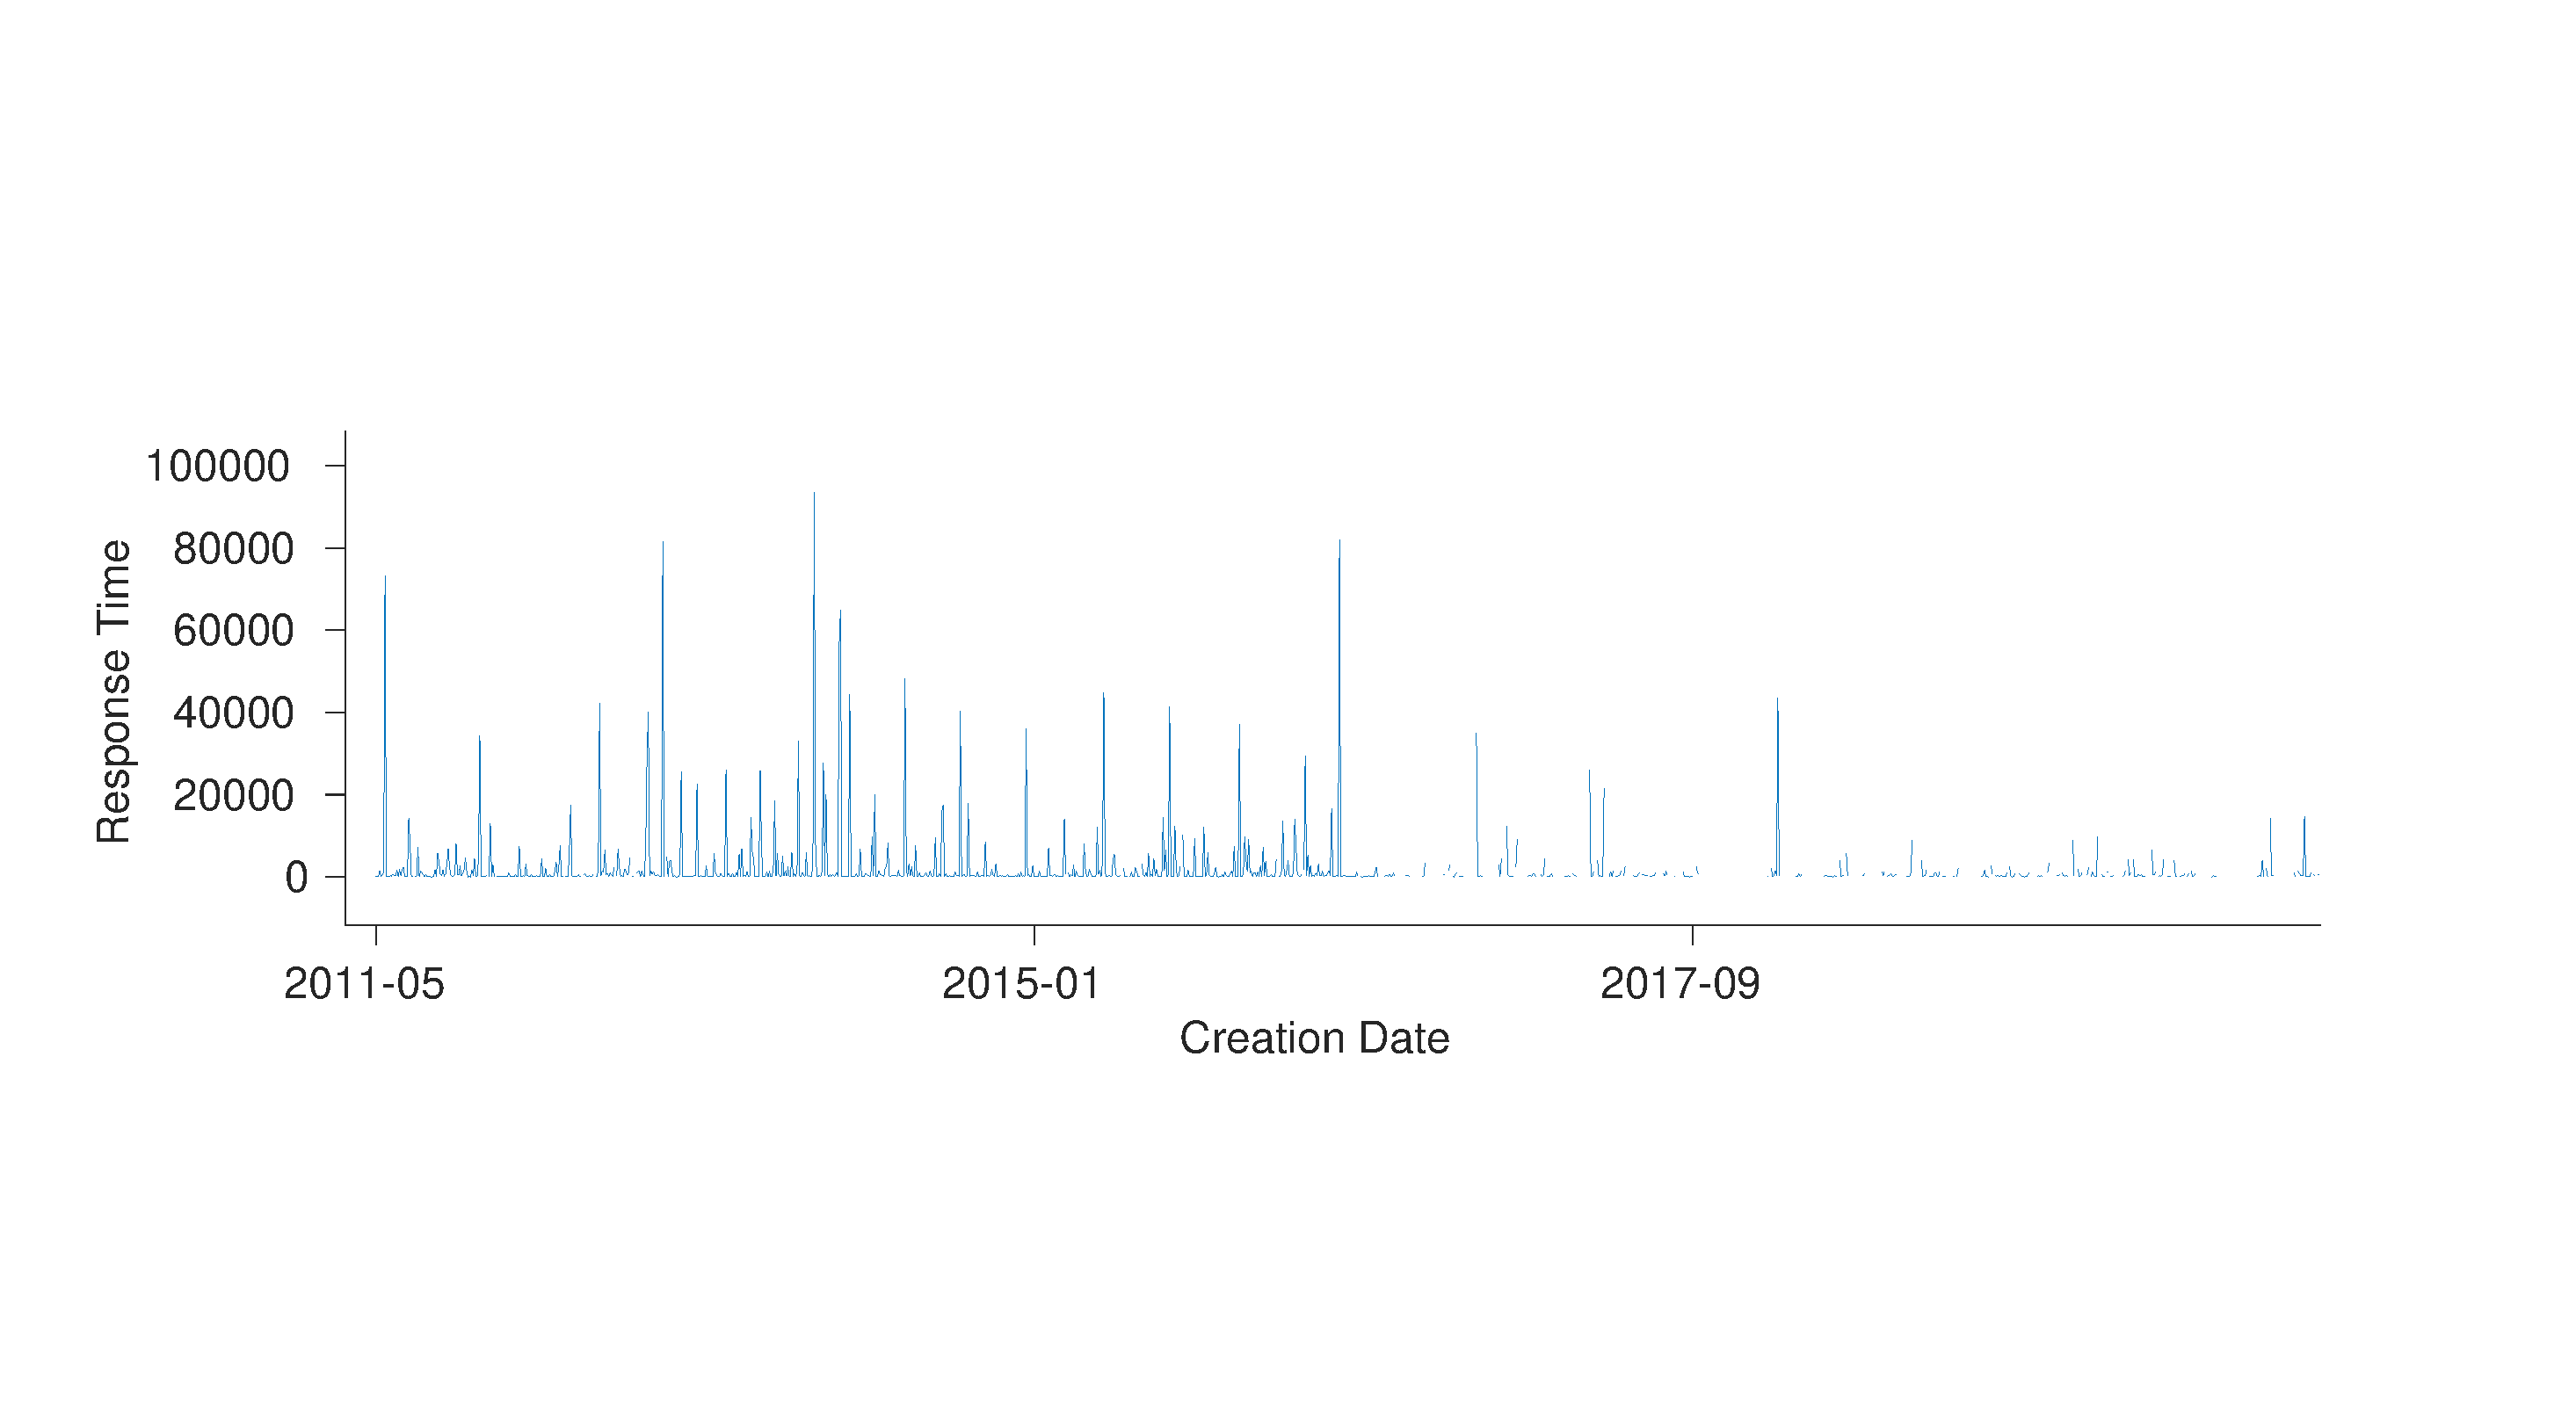
\includegraphics[trim=40 150 120 200,clip,width=1.0\linewidth]{Figures/replacementBinary/plotOutMissStructural_mat}
%       \label{4a}}
%  \vspace{1mm}
%  %\subfloat[Utility]{%
%  %     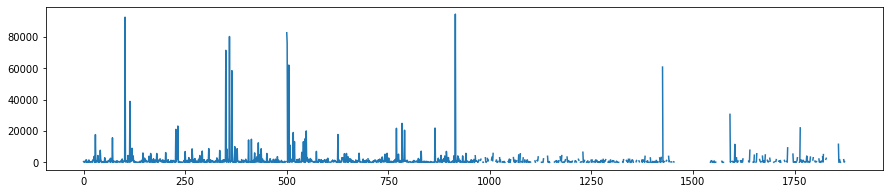
\includegraphics[scale=0.26]{Figures/replacementBinary/plotOutMissUtility.png}
%  %     \label{4b}}
%	\caption{Graphical location in time of outlier and missing values}
%  \label{fig:missingValues} 
%  \vspace{-1mm}
%\end{figure}




%The response time of an event is estimated by the difference between the close date and the creation date of it. Figure \ref{fig:subtype} shows the distribution of reponse time for some subtypes of the groups of events we choose for this work. Although the range of these distributions are wide, our model accomplishes to estimate a response time more accurate that the baselines we use. 
%Together with a model to determine when the next event would occur, this model can support assignment of resources and logistics decisions to improve response for future events.

\section{Problem Statement and Model}
\label{sec:model}
%!TEX root = paper.tex

In this section, we first discuss the future resolution time prediction problem studied in this paper and then describe DeepER, a deep learning based system that predicts future resolution time based on past data.  



\subsection{Problem Statement}
Our aim is to design a system that accurately predicts future resolution times of incidents from historical data. For this purpose, we cast the problem as a time series prediction problem.  We consider a sequence of $n$ events with resolution times X = {$x_1$ , $x_2$ ..... $x_n$}, and predict the resolution time of the next $k$ events Y={ $y_{1}$, $y_{2}$, ..... $y_{k}$}.  What makes this problem challenging and different from classic time series prediction problems is that though these events occur chronologically, the actual time elapsed between two consecutive events varies. This is because each event corresponds to an emergency (i.e., unplanned)  and thus the time when it occurs is completely random. Hence, in some cases one may have considerable time between two consecutive events, whereas in other cases multiple events can occur in a short duration of time. Therefore, our goal is to design a flexible model that examines the resolution time of a sequence of prior events and predicts the resolution time of future events and does not depend on the actual time frame in which the events occurred.


%and then explain the implementation details including hyperparameter selection.

%Figure \ref{fig:preprocessing} shows the system architecture of DeepER. As discussed in the previous section, the data is separated into four datasets based on the incident type --- \textit{Fire}, Law, Structural and Utility. We run our model on these four datasets to get future response time predictions.

%\begin{figure}[!ht]
%    \centering
%       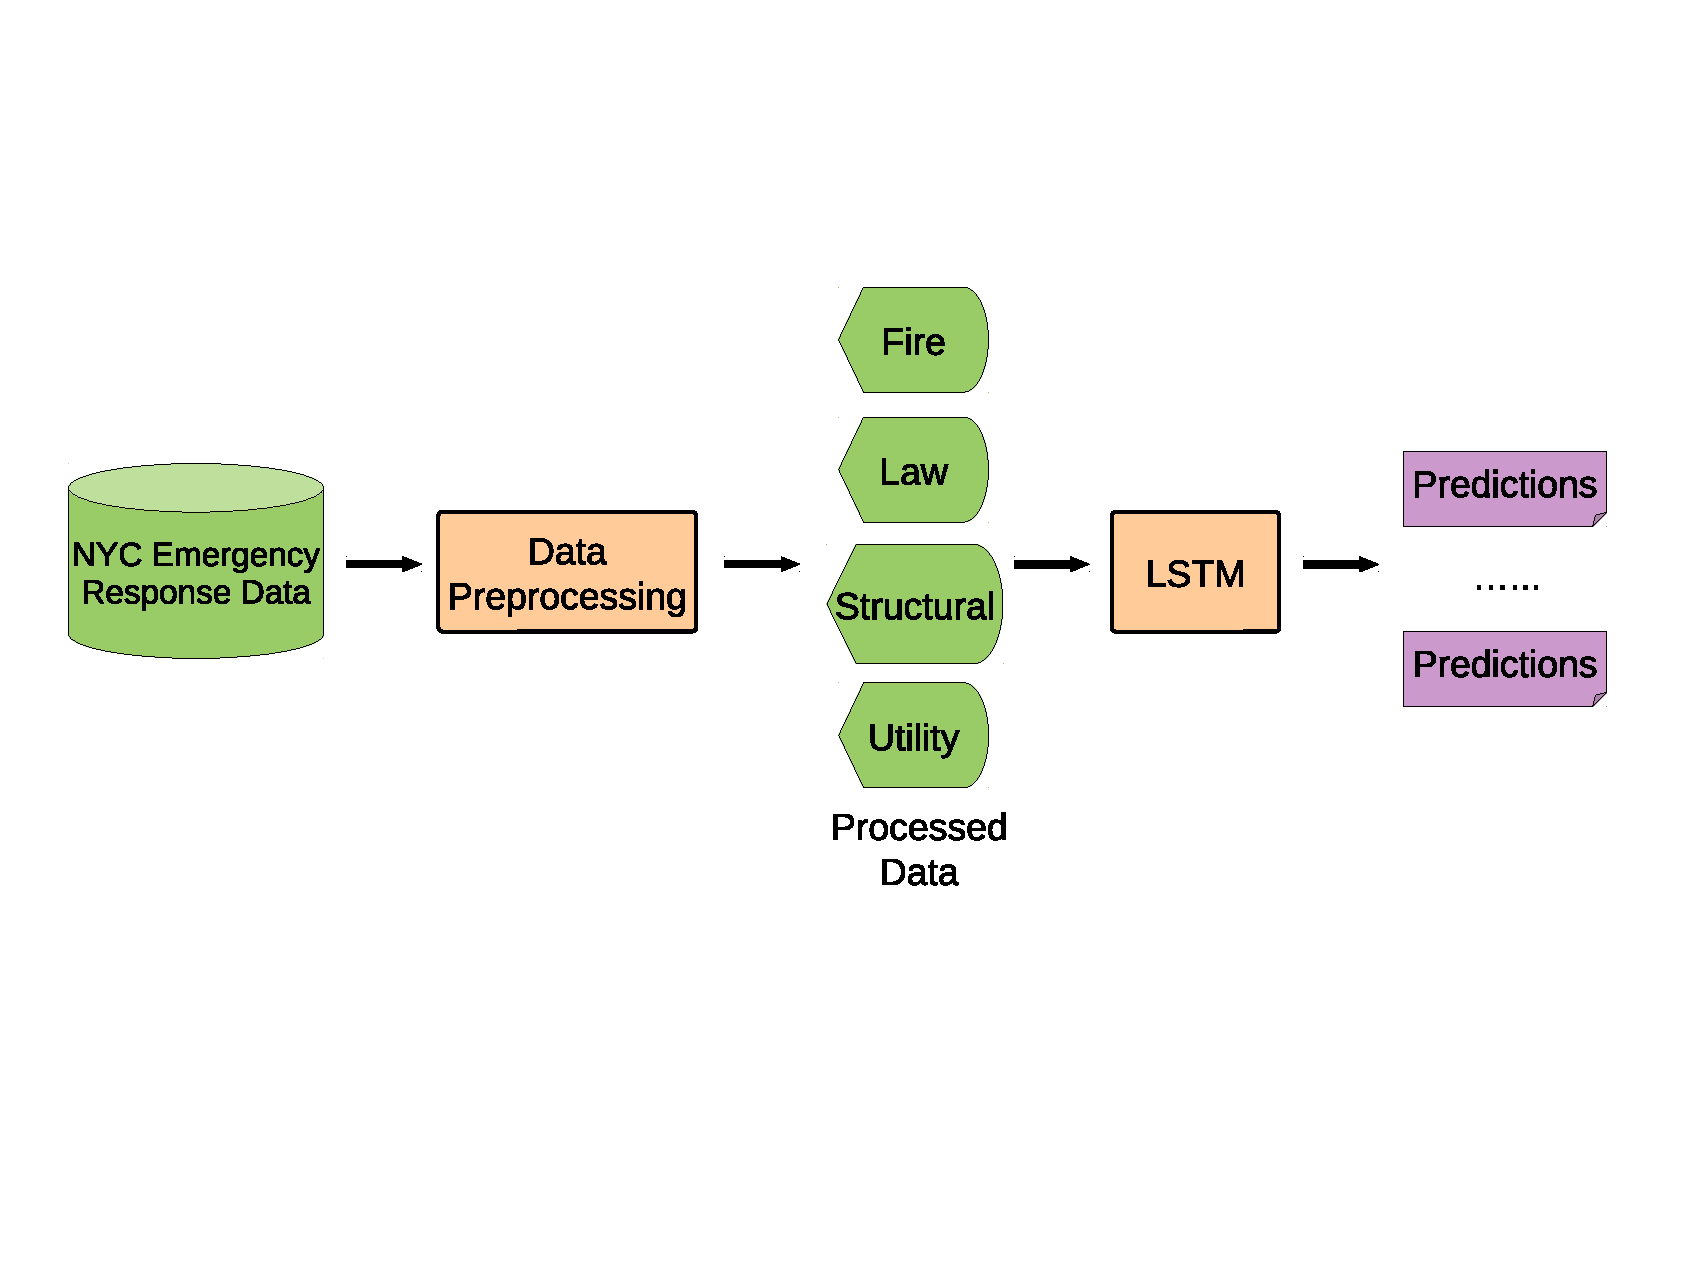
\includegraphics[trim=10 90 10 50,clip,width=1.0\linewidth]{Figures/Model/System}
%       \caption{Architecture}
%  \label{fig:architecture} 
%\end{figure}
%[trim=10 90 10 50,clip,width=1.0\linewidth]{


\begin{figure*}[!ht]
    \centering
       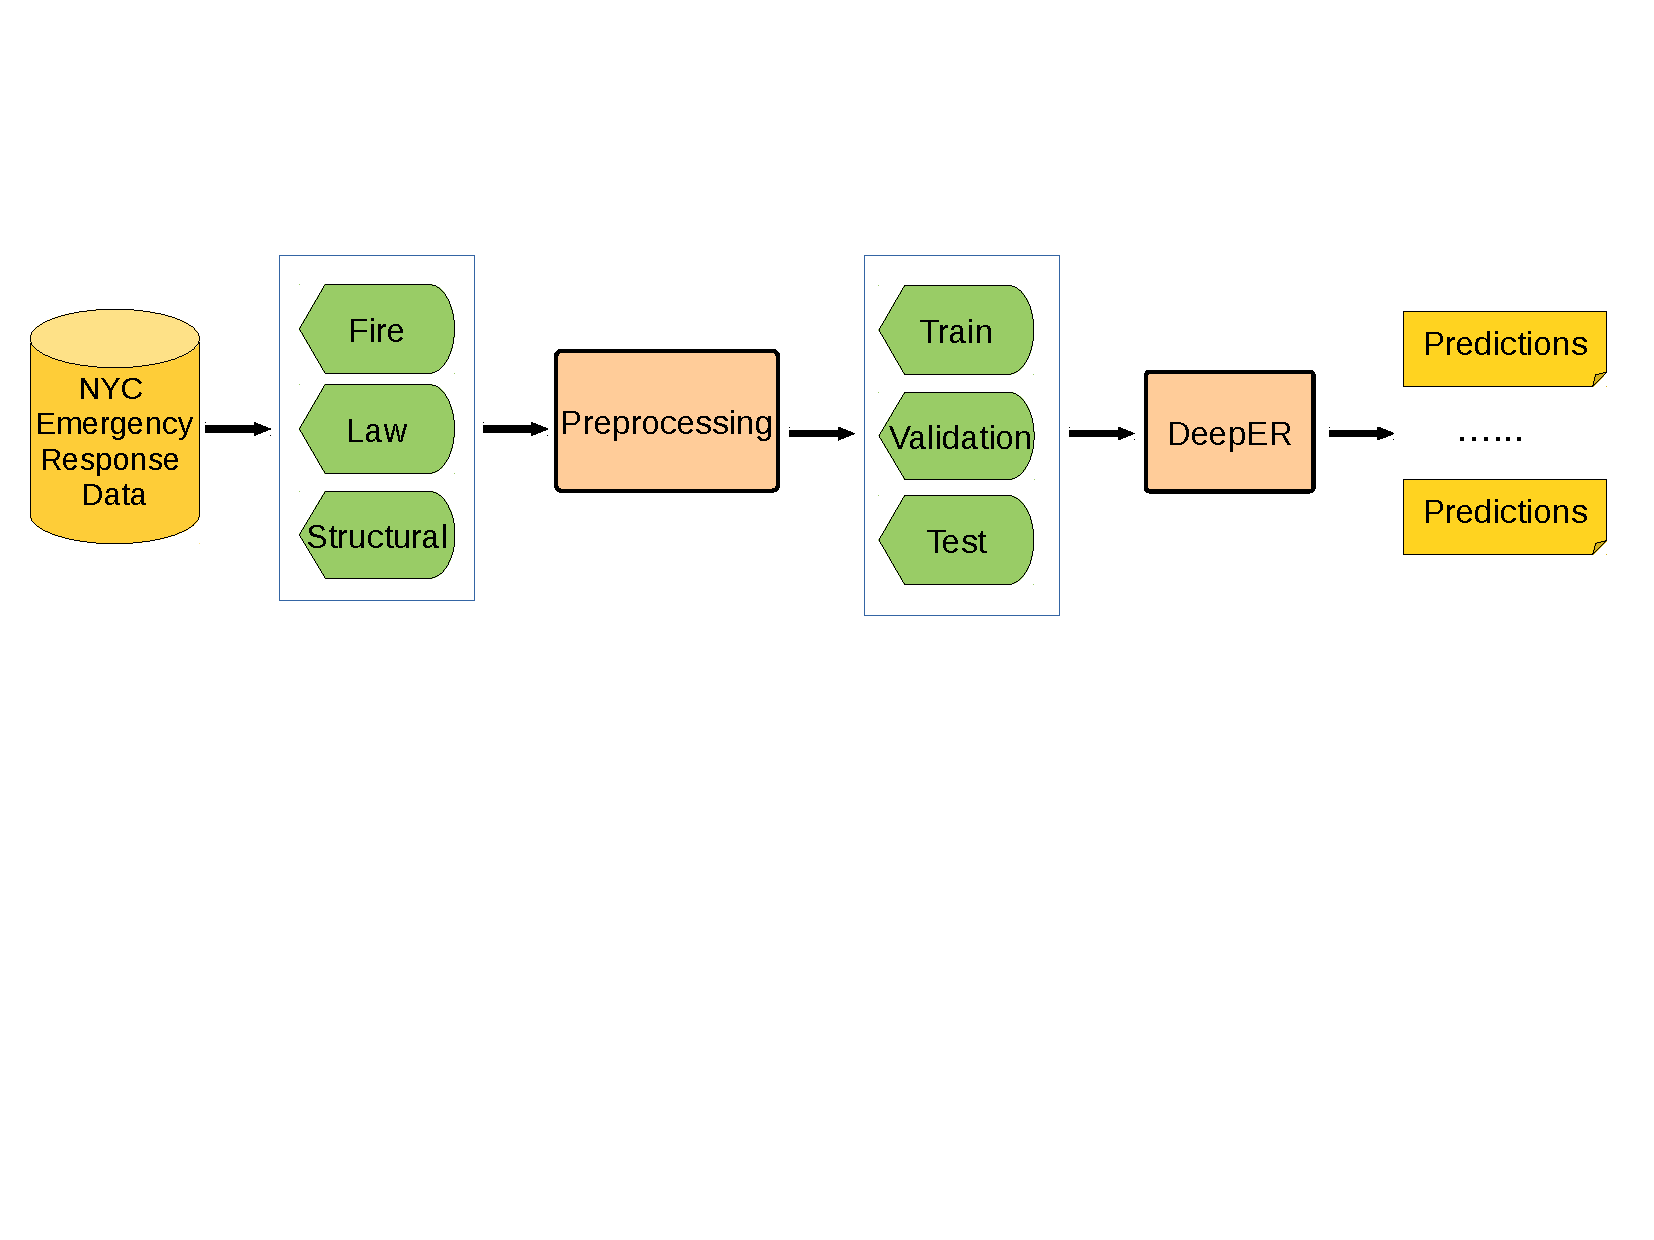
\includegraphics[trim=10 270 10 100,clip,scale = 0.37]{Figures/Model/preprocessing} %width=1.0\linewidth]
       \caption{DeepER System Overview}
  \label{fig:system} 
  \vspace{-3mm}
\end{figure*}



\subsection{DeepER System Details}

In this subsection, we describe DeepER, a sequence-to-sequence based encoder-decoder model that considers the resolution times of  a sequence of prior events to predict the resolution time of future events.   
Figure \ref{fig:system} provides an overview of the DeepER system. \textcolor{blue}{DeepER consists of data preprocessing block that splits the data by incidents and replaces  the outlier and missing values according to the steps outlined in Section \ref{Data:Preprocessing}. The system then splits the data into training, validation, and test (details in Section \ref{sec:implementation}) and then provides it as input to the deep learning model that uses them to generate the predictions.}

%DeepER consists of data preprocessing block that splits the data by incidents and years. The system then splits the data into training, validation, and test (details in Section \ref{sec:implementation}) and replaces  the outlier and missing values with valid points from the training set, according to the steps outlined in Section \ref{Data:Preprocessing}. Finally, the sets are provided as input to the deep learning model that uses them to generate the predictions.


\subsubsection{Sequence-to-Sequence Models}
Before delving into the system details, we discuss the appropriateness of sequence-to-sequence models for the emergency resolution time prediction problem studied here. In comparison to classic statistical regression models, sequence-to-sequence models are  better suited for this problem  as they map entire input sequences to output sequences and do not just  focus on capturing simple trends in the data. Additionally, as the points in the dataset are not  equally spaced in time and the events lack a seasonal and periodic behavioral pattern, we design deep learning based sequence-to-sequence models because such models are capable of learning the underlying dependencies and correlations in the data using an interconnected neural network architecture during the training phase and are especially useful when the dependencies are not apparent and cannot be easily defined. The trained model  leverages this knowledge to make accurate predictions at test time by considering the current input sequence.


\begin{figure}[!ht]
    \centering
       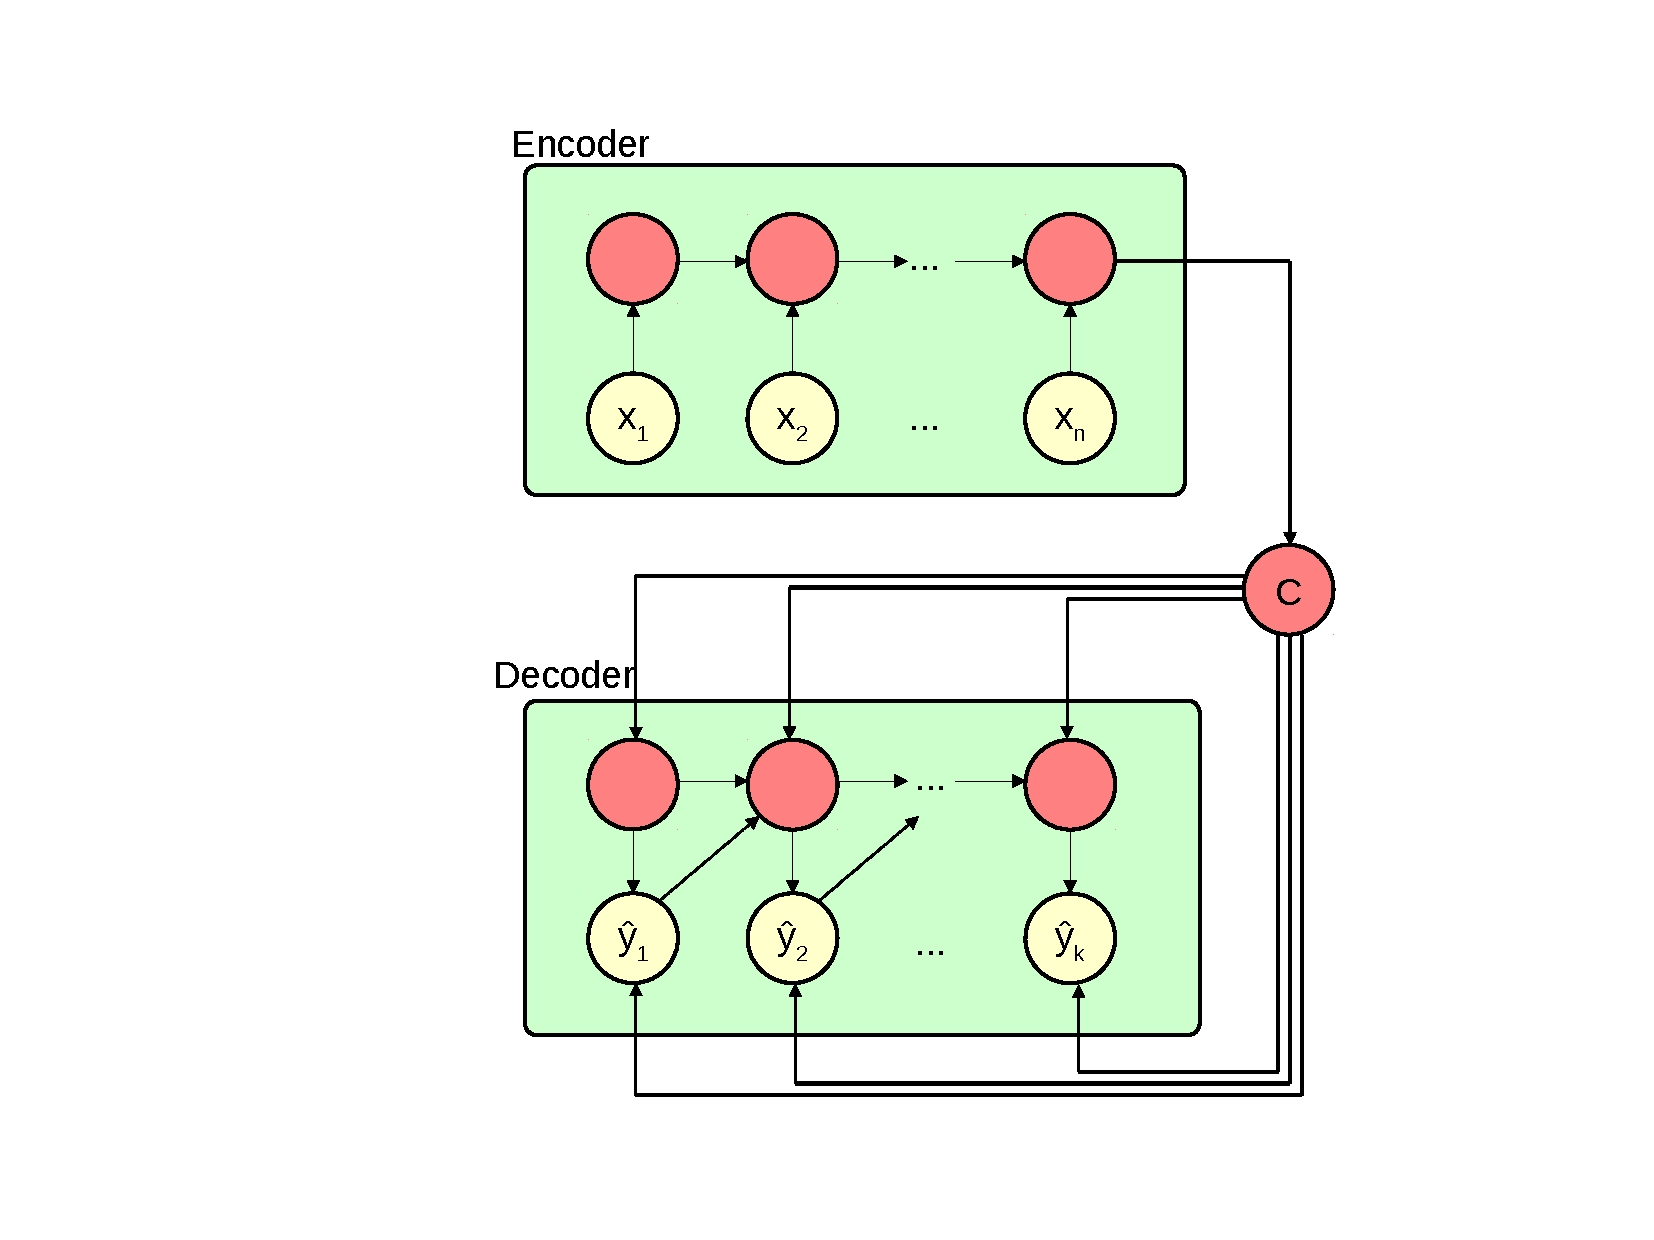
\includegraphics[trim=80 50 10 50,clip,width=1.0\linewidth]{Figures/Model/RNN}
       \caption{Encoder-decoder based RNN}
  \label{fig:RNN} 
\vspace{-3mm}
\end{figure}

\subsubsection{Encoder-decoder based RNN Model}
DeepER consists of two components, an encoder and a decoder as shown in Figure \ref{fig:RNN}. Both the encoder and the decoder comprise of recurrent neural networks (RNN). An RNN is a network of neural nodes that are arranged in layers.  Internally, the RNN has a hidden state $h_t$ that is updated at each time step $t$ using the input $x_t$ and the previous hidden state $h_{t-1}$.    At each time step $t$, the hidden state of the RNN is given by,
\begin{align}
\label{eqn:rnn}
h_t = \phi(h_{t-1}, x_t)
\end{align}
where, $\phi$ is any non-linear activation function and $1$ $\leq$ $t$ $\leq$ $n$.

As we can observe from Figure \ref{fig:RNN}, the encoder takes an input sequence $x_1$, $x_2$, ...., $x_n$ that corresponds to the resolution time of events for the last   $n$ time steps. The encoder then generates a hidden encoded vector $C$. After the entire input has been processed, the summary $C$ is provided as input to the decoder. The decoder then  generates $\hat{y}_1$, $\hat{y}_2$, ...., $\hat{y}_k$, the predicted resolution times for the future $k$ events. \textcolor{blue}{The loss function used is the sigmoid activation function and it is applied to the output of the decoder. This ensures that the predicted values are in the [0-1] range that are later inversely transformed to the original values.}

The basic cell structure used in the encoder is LSTM that captures the important dependencies in the data. LSTM cells also possess the ability to `forget' that enables them to overcome well-known vanishing/exploding gradient. To achieve this an LSTM cell has three main gates---input, output, and forget. The input gate receives the pertinent information in the current step and the output gate determines the hidden state for the next step. The forget gate is responsible for discarding unimportant information so that the model can capture the relevant long-term dependencies. We refer the reader to \cite{cho2014learning, sutskever2014sequence} for additional details.


\section{Implementation Details}
\label{sec:implementation}

In this section, we discuss implementation details regarding training, validation, and testing as well as important design   decisions (e.g.,  hyper-parameter selection).



From our discussion in the Section  \ref{Data:Preprocessing}, we observe that missing points and outliers are not spread uniformly throughout the duration of the dataset. Additionally, the entire duration of the dataset is approximately nine years and therefore, we observe gradual changes in the average resolution times of events for the same incident type. We attribute these variations to possible changes adopted by  the different emergency management agencies. These issues inherent to the dataset necessitate some important design decisions. As the underlying characteristics of the data change over time, if we adopt a simple approach and split the data chronologically into training and test, then we will end up training solely on the data for the initial few years and testing on the last few years. This is unlikely to provide good performance because the distribution of the test data sequences are  different from the distribution of the training sequences. Hence, we adopt a more careful approach where we ensure representation of data from each year in training, validation, and test datasets. 


\begin{table}[!ht]
\centering
\resizebox{\columnwidth}{!}{
\begin{tabular}{|c|c|c|c|}%|M{1.8cm}|M{1.8cm}|M{1.8cm}|M{1.8cm}|M{1.8cm}|M{1.8cm}|M{1.8cm}|}
\hline
\textbf{Sequence Length} &\textbf{Learning Rate} & \textbf{Units in Hidden Layer}\\\hline
10-3	&0.01	&10	\\\hline
10-3	&0.001	&50	\\\hline
10-3	&0.0001	&100\\\hline
15-5	&0.01	&10	\\\hline
15-5	&0.001	&50	\\\hline
15-5	&0.0001	&100\\\hline

\end{tabular}
}
\vspace{3mm}
\caption{Hypararameter combinations for experiments}
\label{tab:hyperparameter}
\end{table}


To do so, we divide the entire dataset into eight periods: seven periods of one year each and one period of approximately one and half year, approximately. We split each of these years in training, validation, and test sets following the usual percentages of 50\%, 25\%, and 25\%, respectively.  This ensures that the training, validation, and test sets contains data from all the years. Additionally, to remove any form of seasonal dependencies that may exist in the dataset, we permute the split order of training, validation and test within each year.  Such permutation ensures that the training, validation, and test data contain samples from all months of the year; in the absence of such reordering the training data will be confined to primarily the first few months, the validation confined to the middle months, and test containing data from the last few months of each year. In addition to helping in achieving good prediction performance across the entire duration of the dataset across the years, this important pre-processing step also makes our model more readily extensible to real-world deployment as the model is trained on the different variations that may be present in the data.



%%%%Figures from results section - placed here for positioning

\begin{figure*}[!ht]
    \centering
%  \subfloat[Fire]{%
%       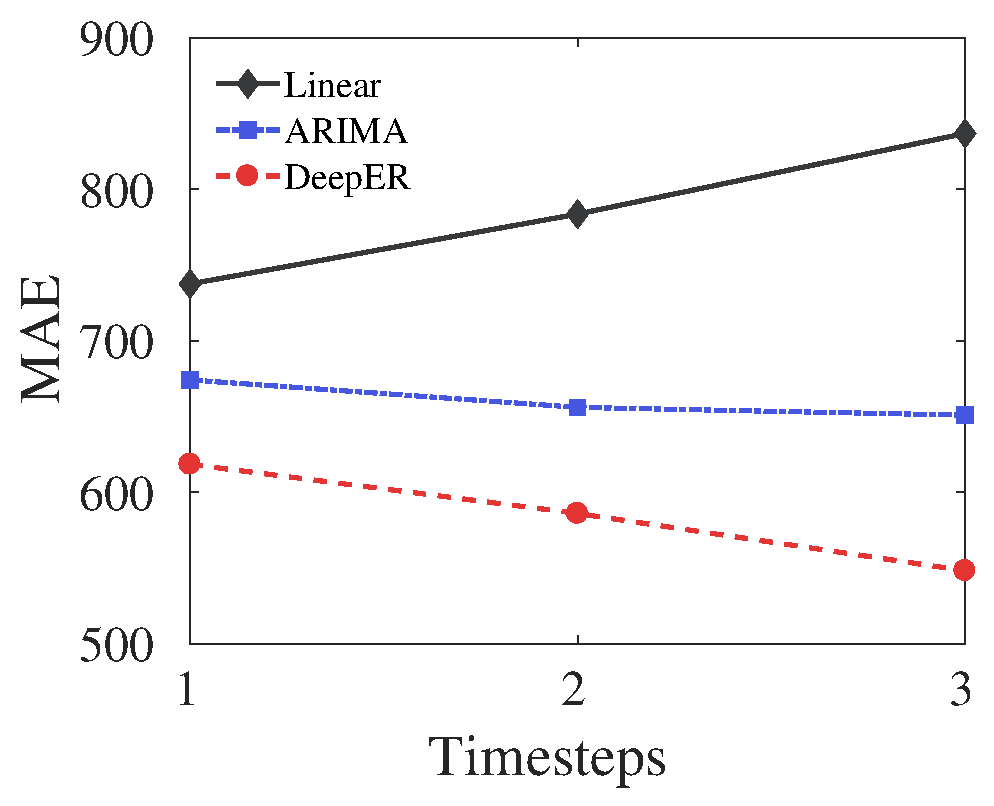
\includegraphics[scale=0.30]{Figures/10_3/Dist/Fire_main_mae_5}
%       }
%  \subfloat[Law]{%
%       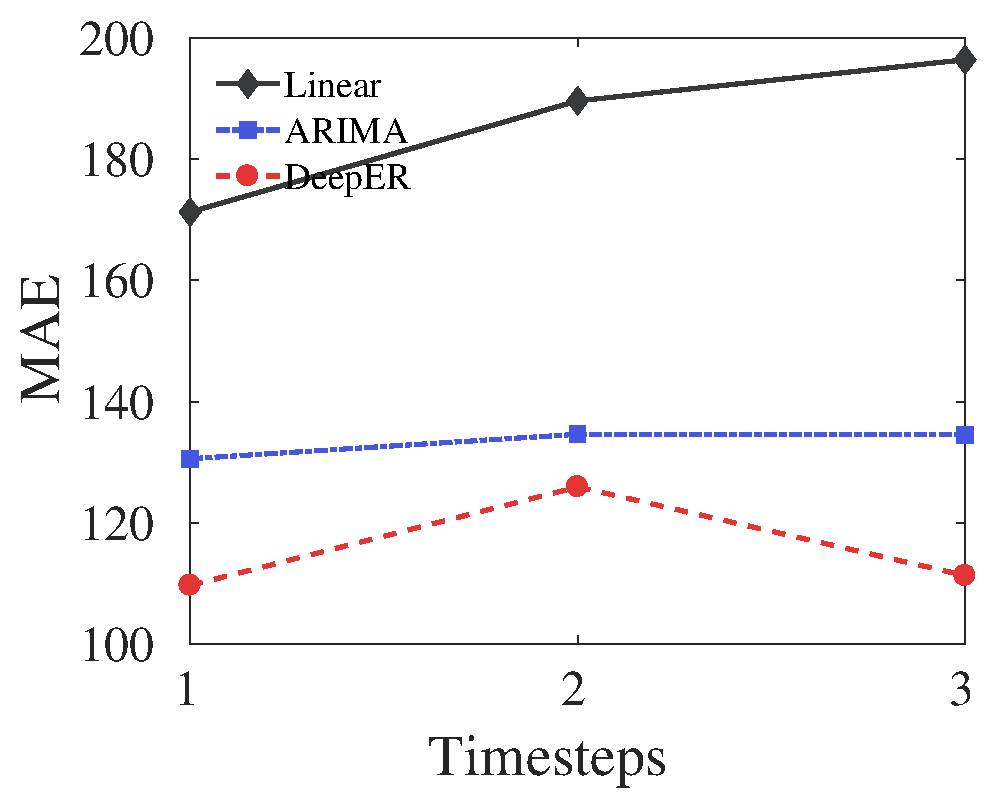
\includegraphics[scale=0.30]{Figures/10_3/Dist/Law_main_mae_6}
%       }
%  \subfloat[Structural]{%
%       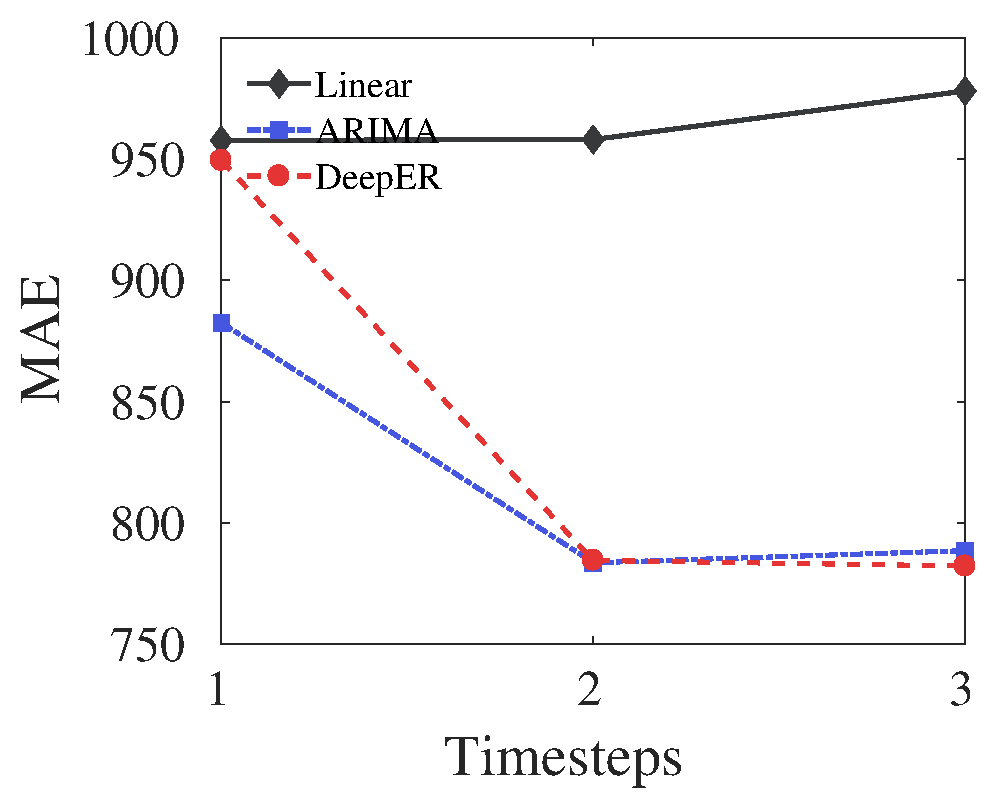
\includegraphics[scale=0.30]{Figures/10_3/Dist/Structural_main_mae_7}
%       }

  \subfloat[Fire]{%
       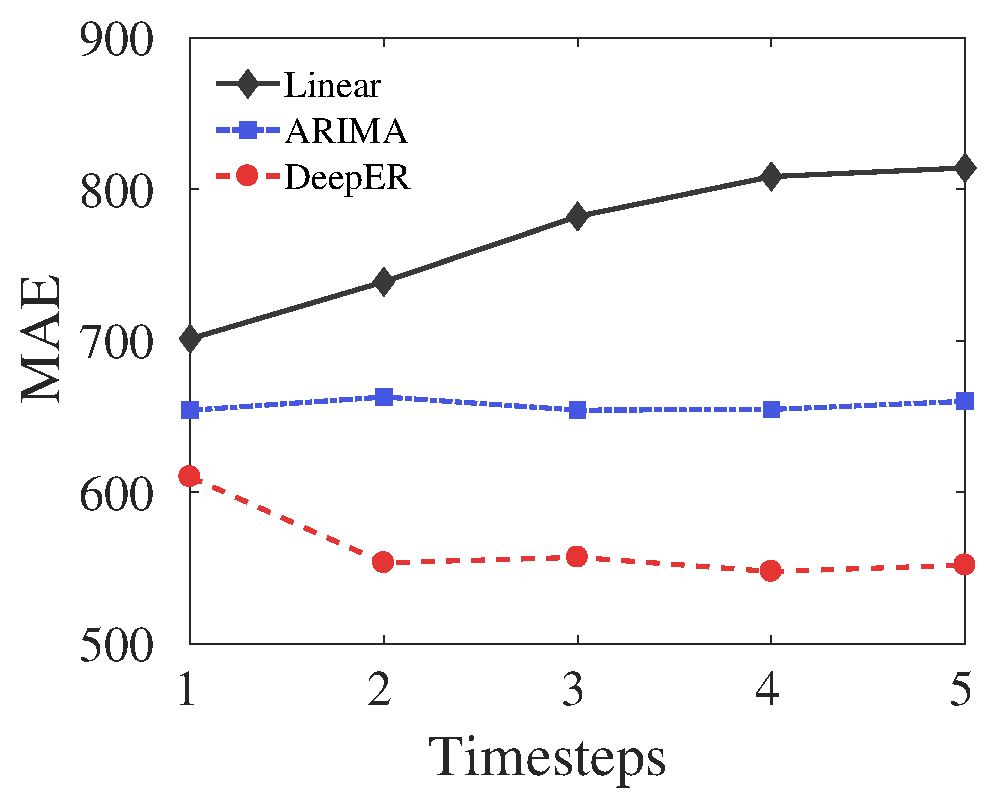
\includegraphics[scale=0.27]{Figures/15_5/Dist/Fire_main_mae_5}
       \label{3a}}
  \subfloat[Law]{%
       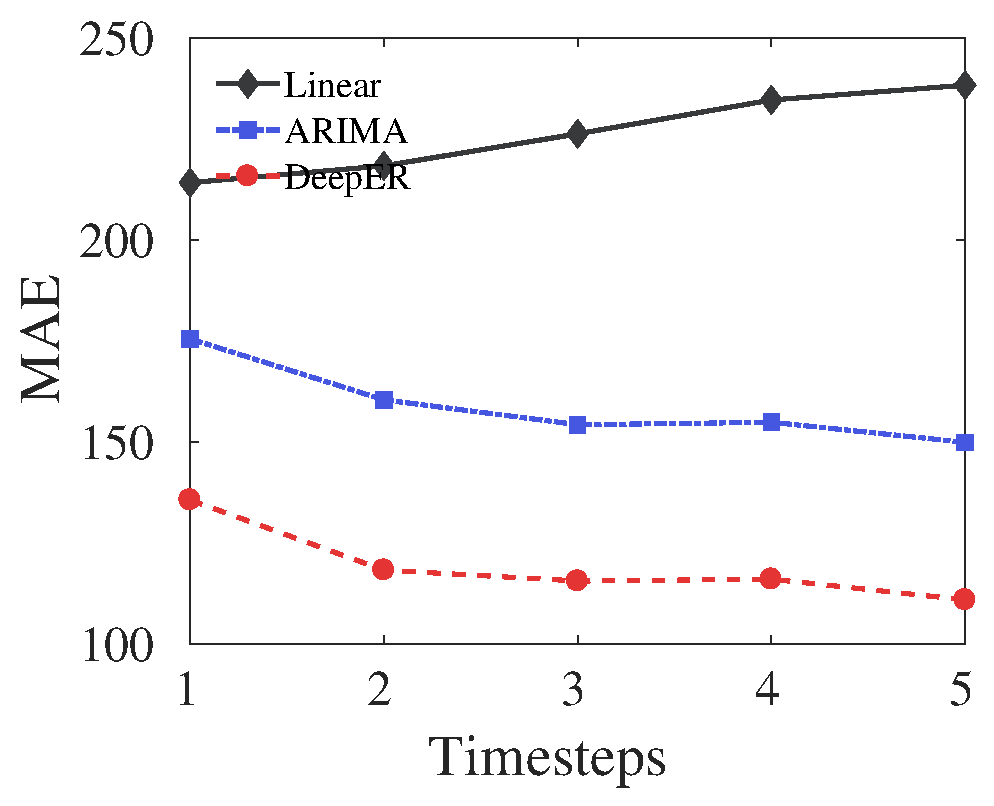
\includegraphics[scale=0.27]{Figures/15_5/Dist/Law_main_mae_6}
       \label{3b}}
  \subfloat[Structural]{%
       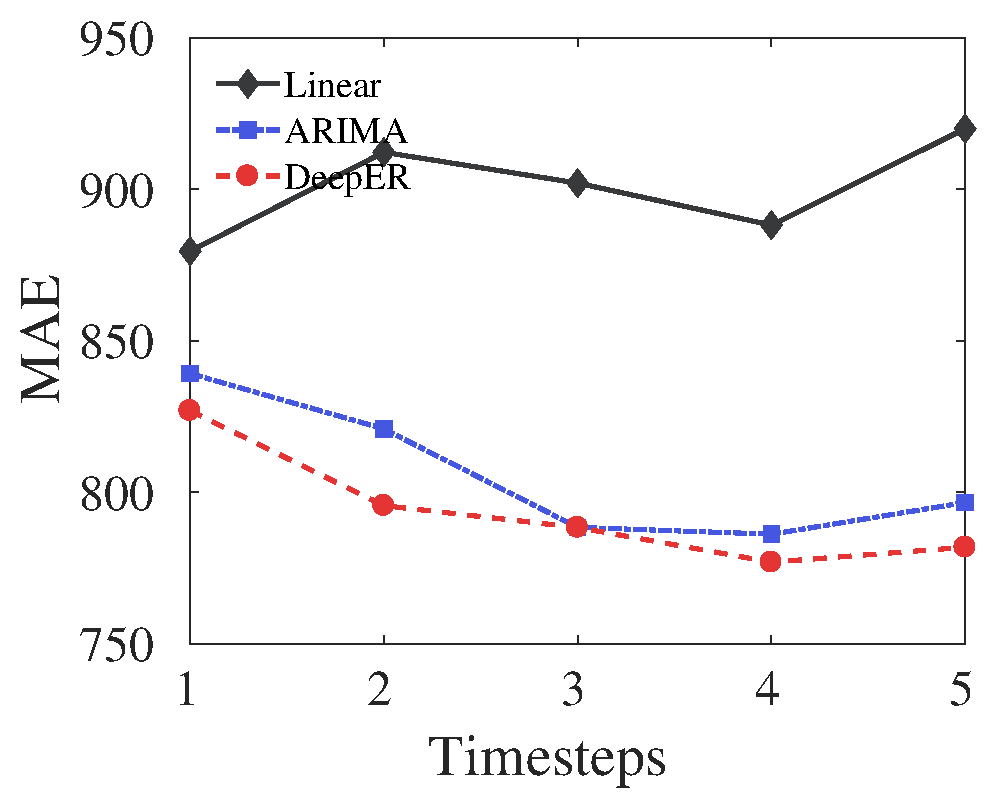
\includegraphics[scale=0.27]{Figures/15_5/Dist/Structural_main_mae_7}
       \label{3c}}
\caption{MAE Results for the 15-5 setting}
  \label{fig:qual_mae} 
  \vspace{-3mm}
\end{figure*}

\begin{figure*}[!ht]
    \centering
%  \subfloat[Fire]{%
%       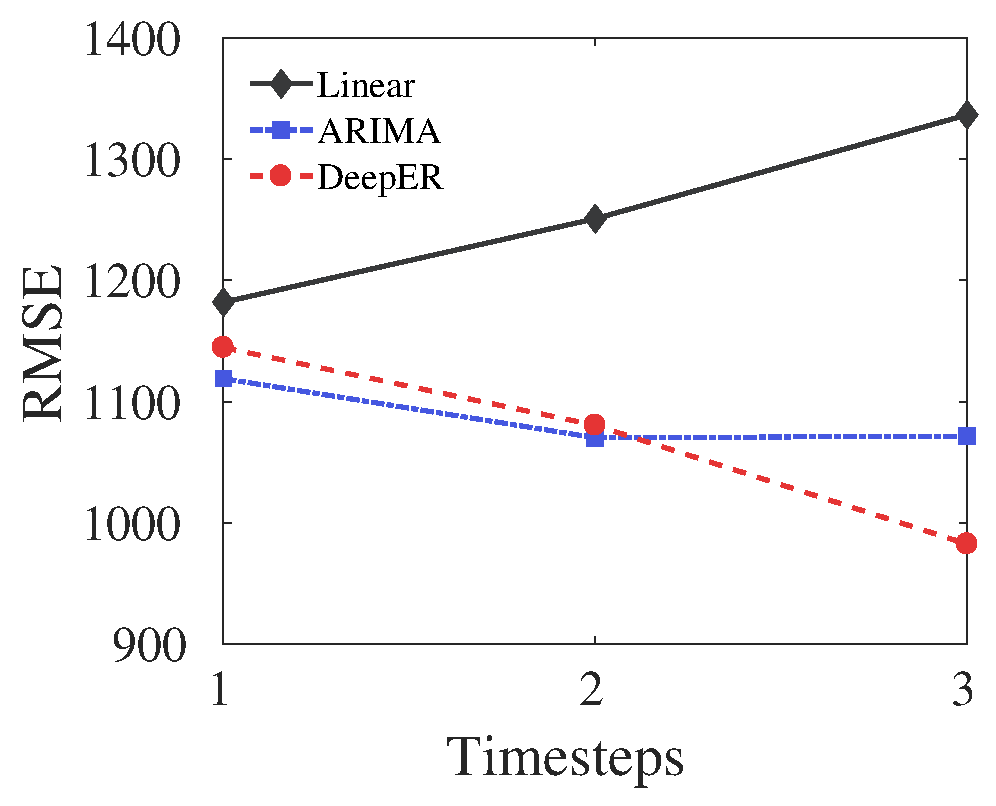
\includegraphics[scale=0.32]{Figures/10_3/Dist/Fire_main_rmse_5}
%       \label{4c}}
%  \subfloat[Law]{%
%       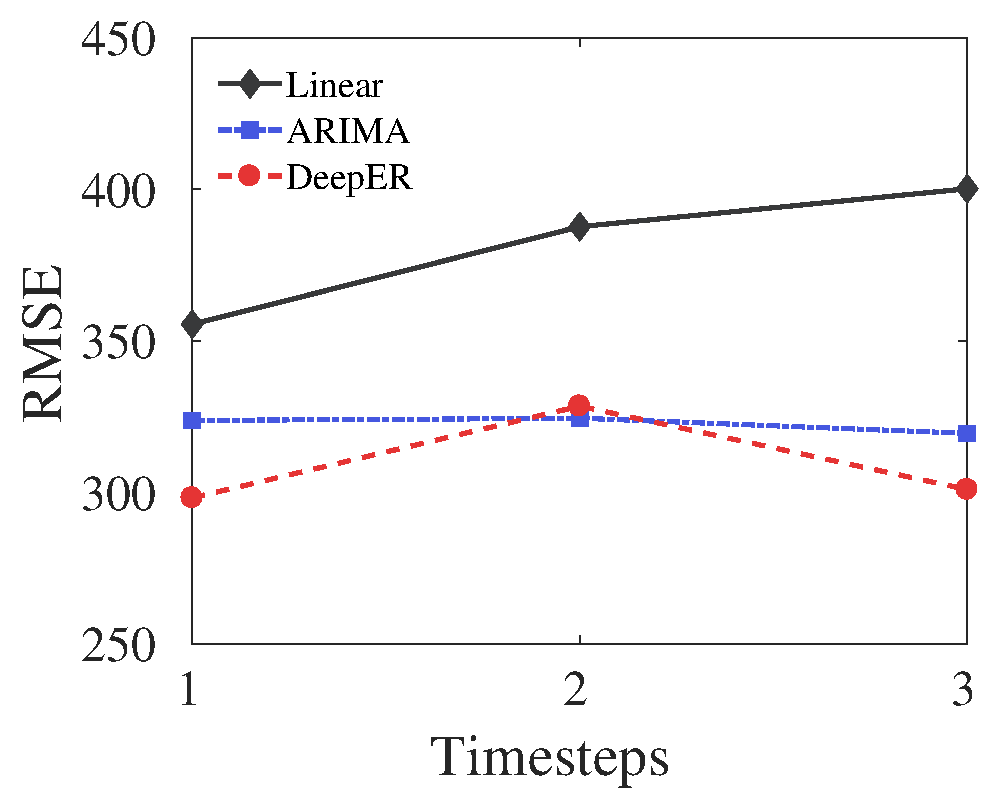
\includegraphics[scale=0.32]{Figures/10_3/Dist/Law_main_rmse_6}
%       \label{4d}}
%  \subfloat[Structural]{%
%       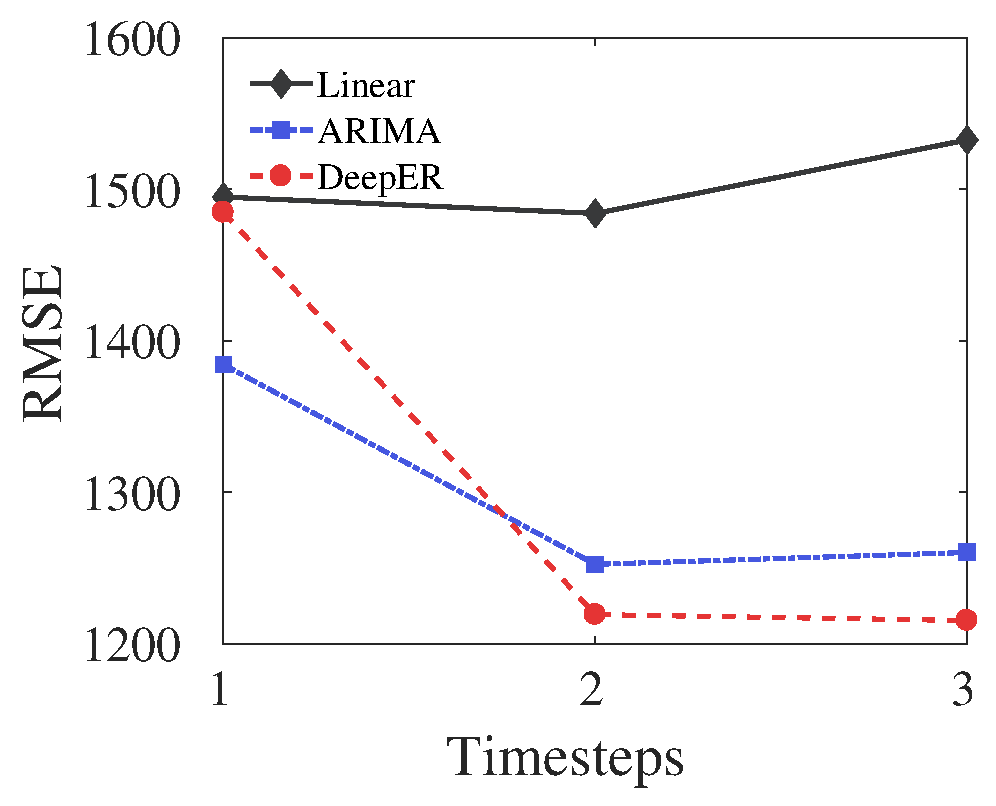
\includegraphics[scale=0.32]{Figures/10_3/Dist/Structural_main_rmse_7}
%       \label{4d}}

  \subfloat[Fire]{%
       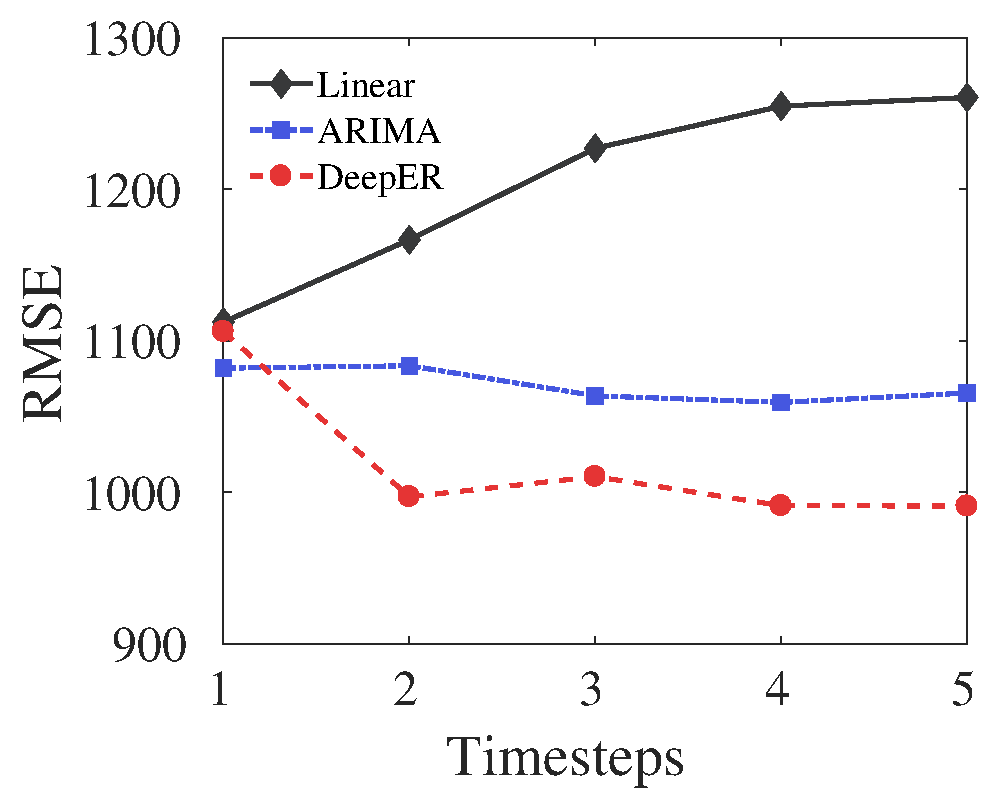
\includegraphics[scale=0.27]{Figures/15_5/Dist/Fire_main_rmse_5}
       \label{4c}}
  \subfloat[Law]{%
       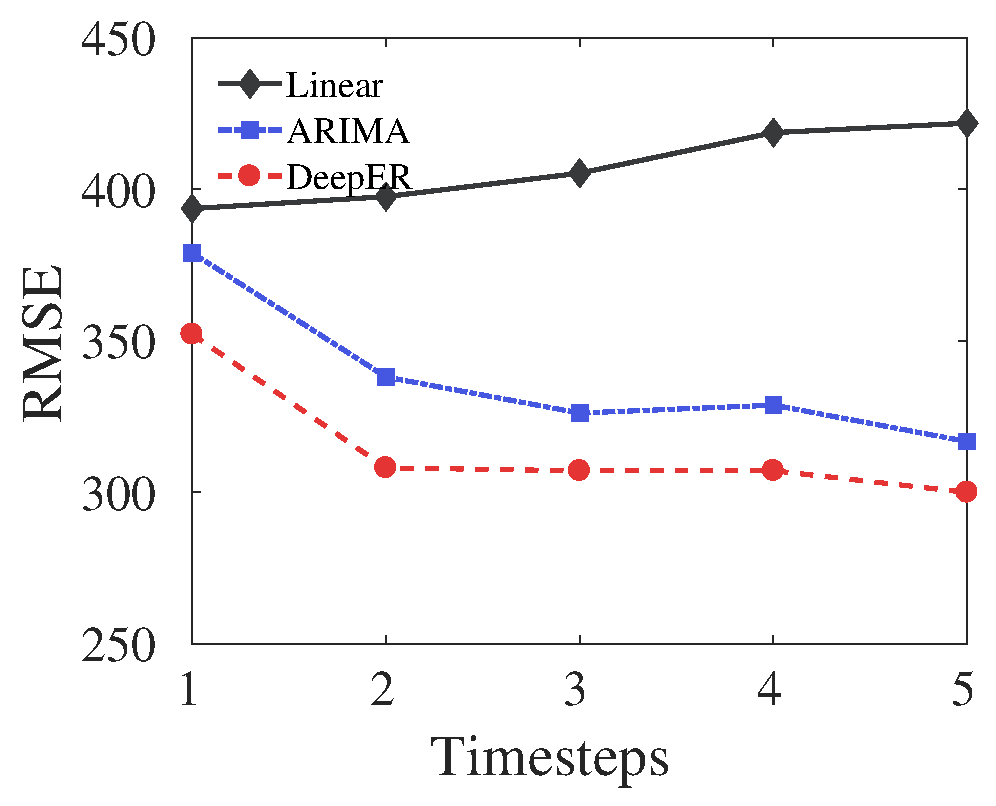
\includegraphics[scale=0.27]{Figures/15_5/Dist/Law_main_rmse_6}
       \label{4d}}
  \subfloat[Structural]{%
       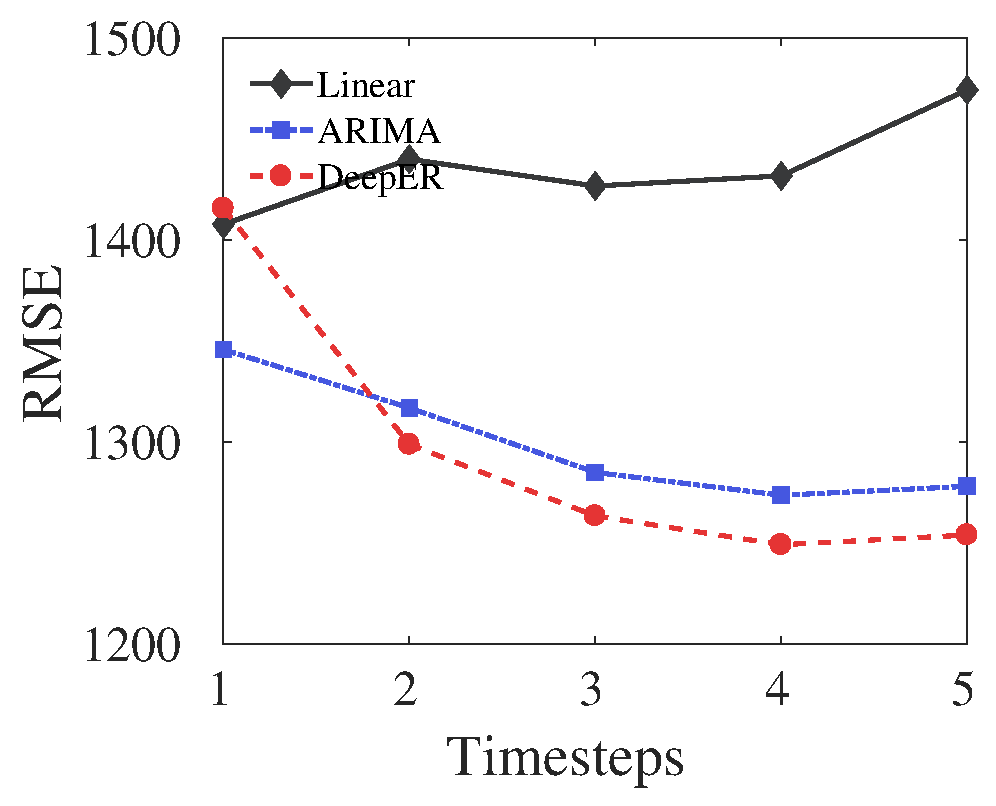
\includegraphics[scale=0.27]{Figures/15_5/Dist/Structural_main_rmse_7}
       \label{4d}}  
  \caption{RMSE Results for the 15-5 setting}
  \label{fig:qual_rmse} 
  \vspace{-3mm}
\end{figure*}

 
%Thus, instead of removing them, we replace the invalid points with the valid points (response times less than quantile 90) from the training set. 



\subsection{Training, Validation, and Testing}
\label{sec:train}

We use Pytorch to implement the deep learning model.   We train our models on a Linux machine with 8-core Intel i7 processor and 64 GB RAM.
%For training our models, we leverage the shared high performance computing cluster available at our university. Using this cluster, we are able to execute multiple experiments in parallel. Each experiment is allocated 4 cores and 4 GB of RAM. %We use the response times for past $m$ events to predict the response times for future $k$ events. %As mentioned before, we split the dataset in 50\% for training, 25\% for validation and 25\% for testing. 
We use a sliding window approach with a stride of 1 to transform the time series into instances of sequences of length $n$ and prediction of length $k$. We use unguided training as the training methodology.  In this approach, the previous predicted output is used by the decoder as an input to the next step of the decoder during both training and test. Unguided approach is likely to provide better results at test time because it allows greater exploration of the state space during training. The loss function used to guide the training is the mean squared error.
% CONFIRM: We use L2 regularization in our model to avoid overfitting.

During the training phase, we experimented with various hyperparameters and then finally decided upon 6 hyperparameter combinations that are best suited for our dataset  (Table \ref{tab:hyperparameter}).  A sequence length of 10-3  in Table \ref{tab:hyperparameter} means that the model takes 10 points are input and predicts 3 points into the future. For each hyperparameter combination, we iterate over 100,000 epochs, saving the state of the model after every 5000 iterations. We then select the particular model combination that provides the best performance on the validation set.  

For quantifying the best performance, we do not simply pick the model with the lowest loss.  Such an approach usually works well when the data has overall less variation and exhibits seasonality. However, in our dataset,  events occur at random times and are of varying intensity (as each event is an emergency), thus resulting in higher variation among the values. \textcolor{blue}{This makes our dataset challenging to predict close to the mean value}. Therefore, in addition to the loss function, we also consider another heuristic, the magnitude of the standard deviation among the predictions on the validation set, to select the best model. This approach ensures that the trained model provides superior quantitative and qualitative performance. Additionally, testing on a validation set and selecting from the myriad of combinations  ensures  that we do not overfit the model to the training dataset. 






%but also the state of the model in which a minimum average standard deviation, among the steps of all predictions, is reached. %, which gives an intuition of the values that are not peaks or where most of the instances lie. 

%we observe that because of the
%We define this criteria in order to ensure our model reaches some variations and does not pick a similar value for all predictions, leading to a close-to-flat line. This minimum value is the quantile 90. We report results evaluating the best model on the test set. 

%We will make available the code for the model and the preprocessing step.
%We experiment with different number of hyperparameters like stacked layers, hidden units, learning rate and number of epochs. We observe that 1 or 2 stacked layers, 5 or 10 hidden units, initial learning rate of 0.01 and the number of epochs ranging between 5000 and 70000 give the best results depending on the incident type. We use exponential decay as the learning rate schedule in our experiments. We augment the model with a feature `sub incident type' in order to improve predictions.

%Figure \ref{fig:preprocessing} shows all the steps in the preprocessing phase. First, we group the dataset by the incident type and then apply the preprocessing steps outlined in Section \ref{Data:Preprocessing}. We then split the dataset into training, validation and test. We then apply the MinMax scale function and transform the dataset into sequences. Such a transformation ensures that all values are in the [0-1] range and is more amiable for manipulation by DeepER. When we evaluate the performance of the model we reapply the transformation to obtain the actual values.


%We calculate some thresholds to replace invalid points. Later applied the MinMax scale function and transform the dataset into sequence instances. Finally, the splits percentages are no exactly the original 50\%, 25\% and 25\% but values near to these ones. This happens due to the cuts among years that, in some cases, trunc the continuation of time steps invalidating instances of lengths $m+k$. We observe that preprocessing does not affect too much the statistics values for Law because it already has smaller values compared to the other incident types. However, the statistics values for Fire and Structural show more perceptible reduction. Additionally, the outlier values before preprocessing, cut off for visualization purposes to 8000 minutes, are much larger than the values after preprocessing.






\section{Experimental Results}
\label{sec:results}
%!TEX root = paper.tex


In this section, we compare the performance of DeepER with two baselines: i) Linear Regression and ii) Auto-Regressive Integrated Moving Average (ARIMA). 

\textit{Linear Regression} is a statistical model that fits the best straight line to the given data. 

\textit{ARIMA} is a statistical model that has three components --- AR (autoregressive term), I (differencing term), and MA (moving average term), specified by the parameters $p$, $d$, and $q$, respectively. We use the \textit{pmdarima} toolkit in python for our experiments, which picks the optimal combination of the parameters for the input data. 

We use two well-known metrics for evaluation---Root Mean Squared Error (RMSE) and Mean Absolute Error (MAE). Equations \ref{eq:RMSE} and \ref{eq:MAE} show how they are calculated, where $y_{ij}$ is the $i^{th}$ test sample for $j^{th}$ time step, $\hat{y}_{ij}$ is the predicted value of $y_{ij}$, and h is the total number of test samples. %We use a third metric based on the number of peaks our model is able to predict. This metric supports the need to predict not only the response time but to know if a coming event would last more than the average value of the events (quantile 50). 
%For the case of \textit{Fire}, an approximation of this thresholds are three days; for Law, 1 day; for Structural, 4 days and for Utility, 2 days.

\begin{equation} 
	\label{eq:RMSE}
	RMSE_{j} = \sqrt{ \frac{\sum_{i=1}^{h} \left( \hat{y}_{ij} - y_{ij}\right)^{2}}{h}}
\end{equation} 

\begin{equation} 
	\label{eq:MAE}
	MAE_{j} = \frac{ \sum_{i=1}^{h} {|\hat{y}_{ij} - y_{ij}|}} {h}
\end{equation}
\vspace{-5mm}


\subsection{RMSE and MAE}


%Predicting response times in such a variational context as different group subtypes and dynamic range time for the sequences instances is not a simple task. The first experiments that we execute, showed lower RMSE values. However, most of them were a flat line prediction. We  modify the optimal value by introducting a condition in the standard deviation. Conditioning the std to be larger than quantile 50, allow our model to learn more variations. 



In this section, we discuss the RMSE and MAE results for all the models. Table \ref{table:dist} shows the average RMSE and MAE results for sequence lengths $10$-$3$ and $15$-$5$, where the average performance is calculated over 3 and 5 time steps, respectively. Recall that a sequence length  $10$-$3$ means that the model takes 10 events as input and predicts 3 events as output into the future. We see that DeepER outperforms the baselines with respect to  both MAE and RMSE for all incident types on average for the $15$-$5$ setting. For the  $10$-$3$ setting,  DeepER outperforms both baselines for \textit{Fire} and \textit{Law}. However, for \textit{Structural}, it outperforms Linear but not ARIMA. Therefore, from Table \ref{table:dist}, we observe that  DeepER   provides overall better performance for the $15$-$5$  setting.

\begin{table}[!ht]
\centering
\resizebox{\columnwidth}{!}{
\begin{tabular}{|c|c|c|c|c|c|}
\hline
\textbf{Incident}&\textbf{Model}&\multicolumn{2}{|c|}{\textbf{10-3}}&\multicolumn{2}{|c|}{\textbf{15-5}}\\
\cline{3-6}
\textbf{Type}&&\textbf{MAE}&\textbf{RMSE}&\textbf{MAE}&\textbf{RMSE}\\
\hline
\multirow{3}{*}{Fire} &Linear& 786 & 1256  & 769 & 1204 \\
&Arima& 660 & 1087  & 657 & 1071\\
&DeepER& \textbf{584} & \textbf{1069} & \textbf{564} &\textbf{1019} \\
\hline
\multirow{3}{*}{Law} &Linear& 186 & 381  & 226 & 407 \\
&Arima& 133 & 323  & 159 & 338 \\
&DeepER& \textbf{116} &\textbf{309}  & \textbf{119} &\textbf{315} \\
\hline
\multirow{3}{*}{Structural} &Linear& 965 & 1504 & 900 & 1436  \\
&Arima & \textbf{818} & \textbf{1299} & 806 & 1300 \\
&DeepER&839&1307  & \textbf{794} & \textbf{1296}\\
\hline
\end{tabular}
}
\caption{Average RMSE}
\label{table:dist}
\vspace{-7mm}
\end{table}



%Additionally, we see that DeepER has lower standard deviation than the baselines. This could be because the baselines try to predict the next time step by replicating the actual signal, accurately predicting the value of peaks while in a shifted manner. This helps us realize the condition for selecting a state in which the standard deviation of the prediction is greater than a minimum value, might not be enough to guarantee more variations in the predictions.
%We discuss this more in \label{Data:Preprocessing}.

Figures \ref{fig:qual_mae} and \ref{fig:qual_rmse} shows the MAE and RMSE results for the three incident types for the 15-5 sequence setting as it provides the best predicitons. We observe that DeepER significantly outperforms the baselines with respect to both MAE and RMSE. The only exception is the one step prediction for \textit{Structural} where DeepER exhibits poor performance. Interestingly, from the figures, we observe that DeepER  is able to better predict  the resolution time of events further into the future. This is in contrast to most time series prediction problems where the prediction performance deteriorates as the model predicts further into the future. The primary reason behind this behavior is that the data points in our dataset correspond to emergency events and hence lack seasonality, strong correlation, and trends. DeepER is still able to generate better predictions for our challenging problem than the baselines because of its sequence-to-sequence behavior that maps entire input sequences to output sequences and ability to glean complex underlying dependencies in the data that are not apparent. 

%With respect to MAE, we observe that DeepER outperforms the baselines among the predicted steps for all incident types for the $15-5$ setting. However, for $10-3$, it outperforms the baselines in all time steps for \textit{Fire} and \textit{Law} but not for \textit{Structural}, where it falls short for the first time step prediction. With respect to RMSE, the figure shows that in most of the time steps, for all incident types and lengths, our model reaches better values, for both lengths settings. However, that is not the case for few time-steps in \textit{Fire} and \textit{Structural} for which we suggest some more analysis in the section of \ref{sec:conclusion}. 



%both lengths and replacing configurations on the two baselines models and our LSTM model. For \textit{Fire} and Law, we get better RMSE with our model. However, for Structural, we get better results except in the 10-3 configuration, in which ARIMA model gets a smaller RMSE. For Utility, ARIMA gets a better RMSE in both lenghts and replacement configurations. We do not observe a significant better performance of one of the replacement configurations compared to the other one, for all group types and lenghts. Nevertheless, we do observe that predicting $5$ time steps based on previous $15$ usually improves the average RMSE, compared to $10-3$. The models that have a better RMSE corresponds respetively to a lowest Standard Deviation. 

%We introduced and external metric (not conditioning the loss funciton) such as the average ratio of peaks predictions. The Linear Regression Model gets the closest value to 1 for thism metric among all group types, length and replacement configurations. This is an interesting metric because it means that among all the prediction time steps $k$, the baselines predict a more similar number of peak values. However, this is a mesleading sense of accuracy and will depend on the final use of the model. If the number of peaks is more important in the prediction lenghts than the actual values or average, this metric can be very useful. Howevere, if it is more important to predict an average of the response time of the coming events, this metric does no play a great role. 



%When analysing the average RMSE we can see how most of the times, our model outperforms the baselines. When we analyse the results with more granularity, per time step, we find out more interesting take aways. Figure \ref{fig:rmse_dist} and \ref{fig:rmse_random} show RMSE results for the multi-step prediction for lengths $5$ and $3$. As expected from the average, we observe from the figures that LSTM outperforms most of the time steps for \textit{Fire} and Law. %We also observe that the RMSE values do not change over time. This is because the events in all incident types do not occur within a certain time interval. Thus, even though there is some pattern learned by the model, the response times of the immediate previous time step does not have significant impact on the current prediction.








\section{Discussion}
\label{Data:Discussion}
%!TEX root = paper.tex



In the previous section, we demonstrated that DeepER provides superior prediction performance than the baseline models. In this section, we discuss some additional learnings from our exploration of this dataset.

\subsection{Qualitative Results}

 We next discuss the qualitative prediction performance of DeepER  as well as the baselines.  Figure \ref{fig:qualitative} shows  the 1-step prediction performance for DeepER, ARIMA, and linear regression for \textit{Fire}.  From the figure, we observe that all models  struggle to predict the values accurately.  From our experience of working with similar models in the past  \cite{SWaP, DeepFit, 8884240}, we have observed that sequence-to-sequence models are generally able to make really superior predictions. This does not appear to be the case always for this prediction task primarily because of the challenging non-periodic and non-seasonal nature  of the emergency events dataset. 
 
 We  observe from Figure \ref{fig:qualitative} that the resolution times for some events is significantly higher in comparison to majority of the points. Because of this pattern, any prediction model  will find it difficult to accurately predict such high peaks. But, despite this  challenging nature of the dataset,  we observe that DeepER   provides a significantly smoothened prediction performance in comparison to the baselines and accurately predicts the underlying pattern. If we overlook the peaks, we can see that  the prediction performance of DeepER for the remaining data points is good. 
 
 In comparison, we observe that the next step predictions for both ARIMA and Linear Regression closely mirror the  actual resolution time  of the previous time step. This occurs because both these baselines only use the past trend to predict the future. This is the root cause behind their poor performance because the  resolution time of the current request is significantly different from the previous one.
 
% As discussed before, due to the events not occurring in fixed time intervals, it is difficult to learn the exact pattern for this dataset.% and hence the predictions do not perfectly match the actual response times, but they try hard to learn the variational patterns from the data. %As mentioned in Section \ref{sec:data}, each incident type has between 29 and 73 sub types. These sub types have response times in different ranges. This leads to high variation in data. Also, as emergency events do not occur in a fixed pattern, the response times are recorded as the incidents are encountered and they are not in fixed time intervals. 

%Besides, the variation in the data due to peaks representing large response times and occurrence of incidents in dynamic length intervals makes forecasting a challenging task. Though DeepER does not accurately predict all the actual response times as seen in Figure \ref{fig:qualitative}, it does predict in a more consistent manner trying to learn the pattern given the complexity of the dataset.



%\begin{figure}[!ht]
%  \centering
%  \subfloat[Fire]{%
%  	\label{fig:qualfire}
%       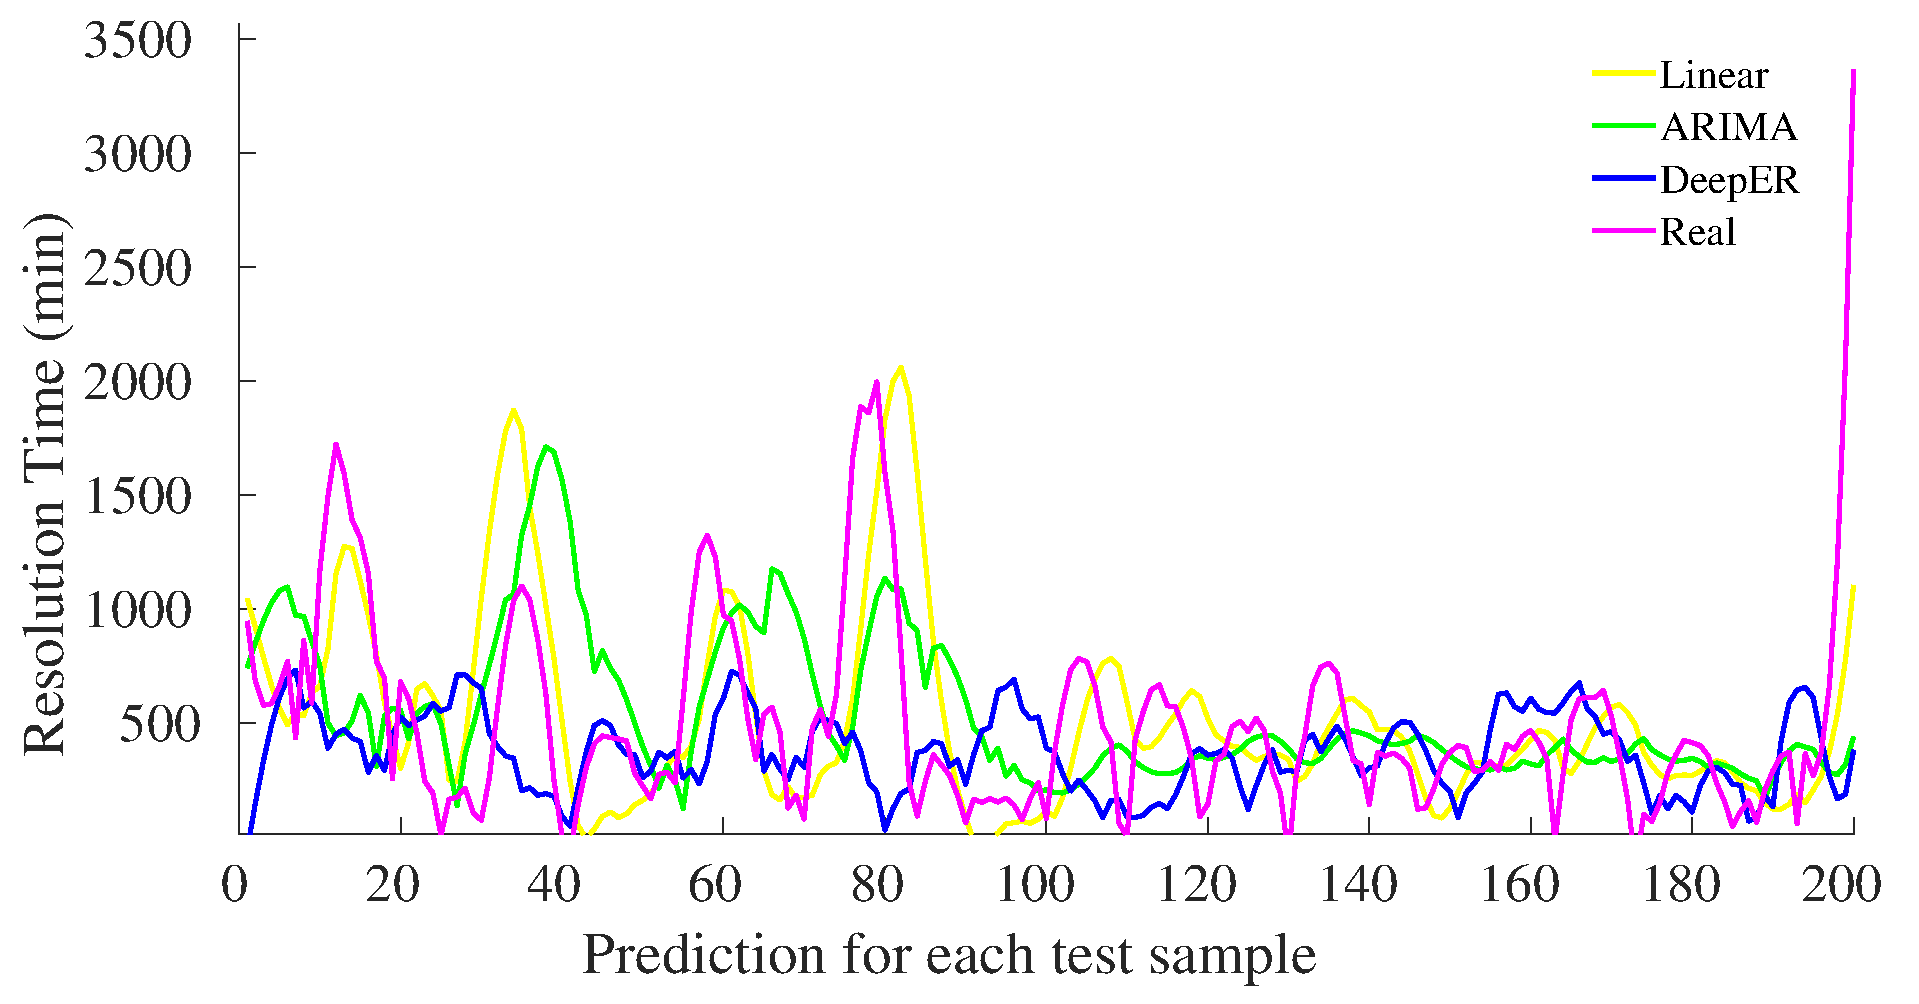
\includegraphics[width=0.9\columnwidth]{Figures/15_5/Dist/1Fire_main_5}
%       }
%  \hfill
%    \subfloat[Law]{%
%         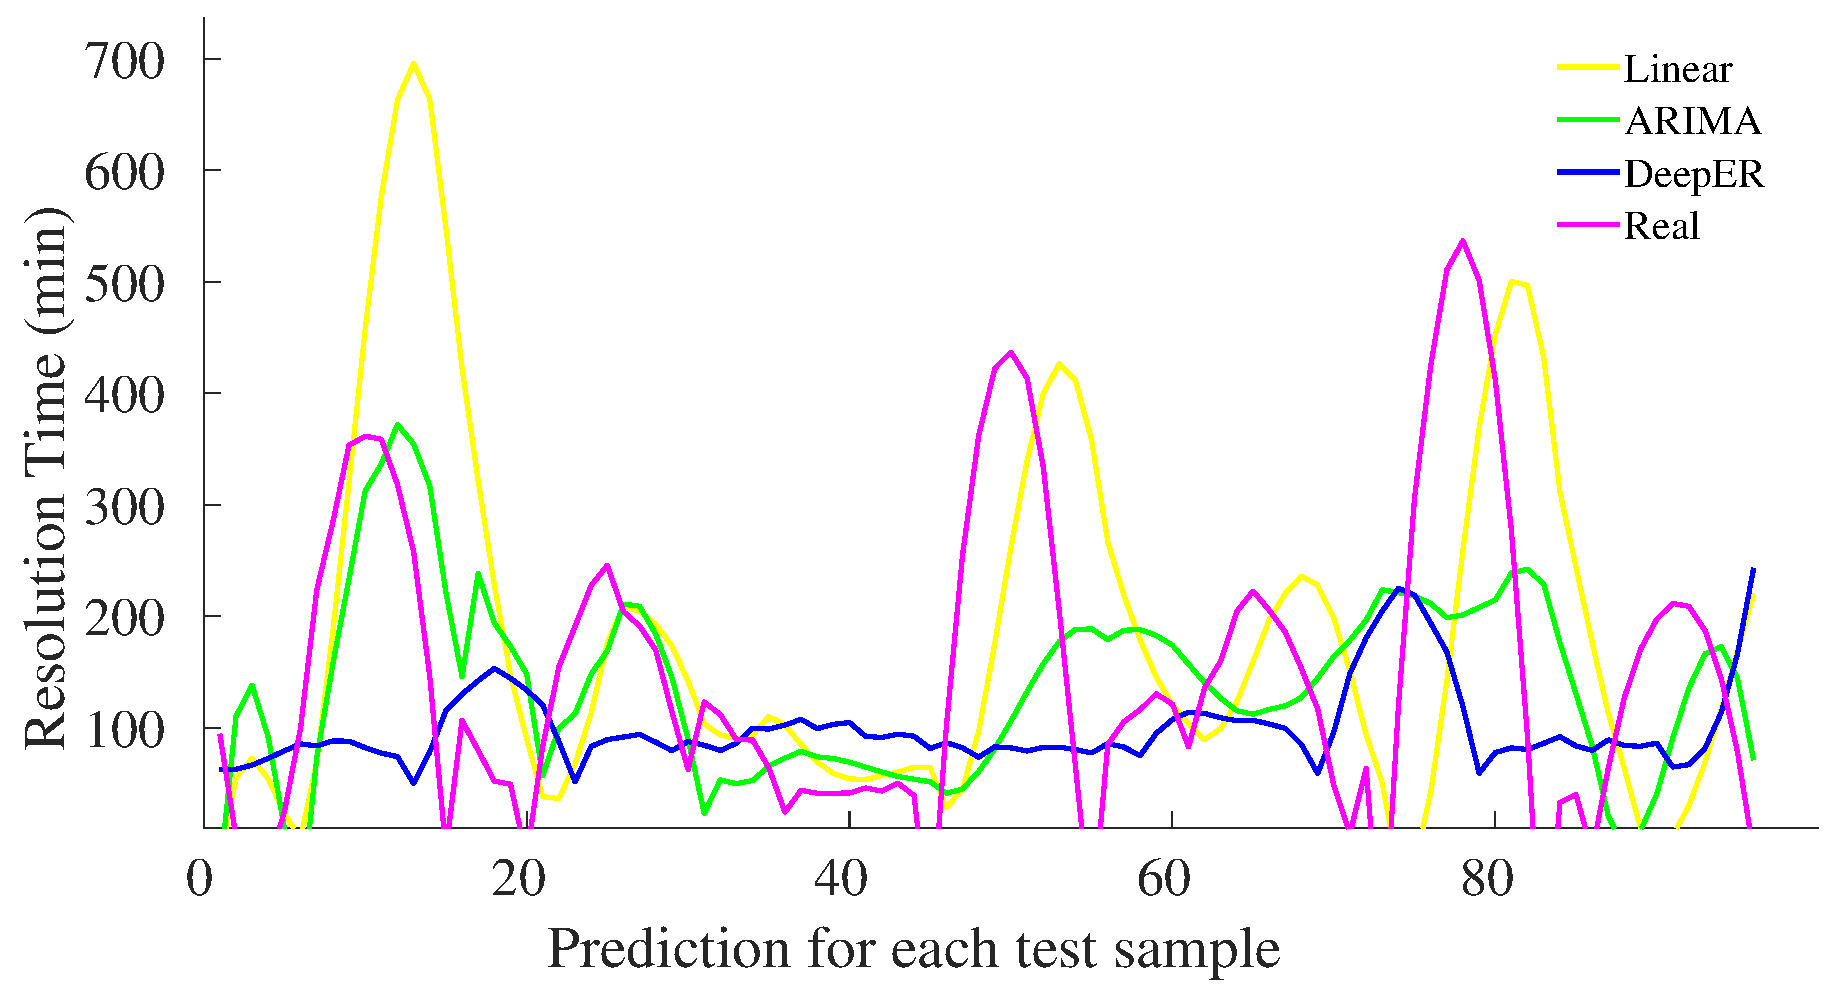
\includegraphics[width=0.9\columnwidth]{Figures/15_5/Dist/1Law_main_6}
%         \label{5b}}
%    \hfill
%  \subfloat[Structural]{%
%       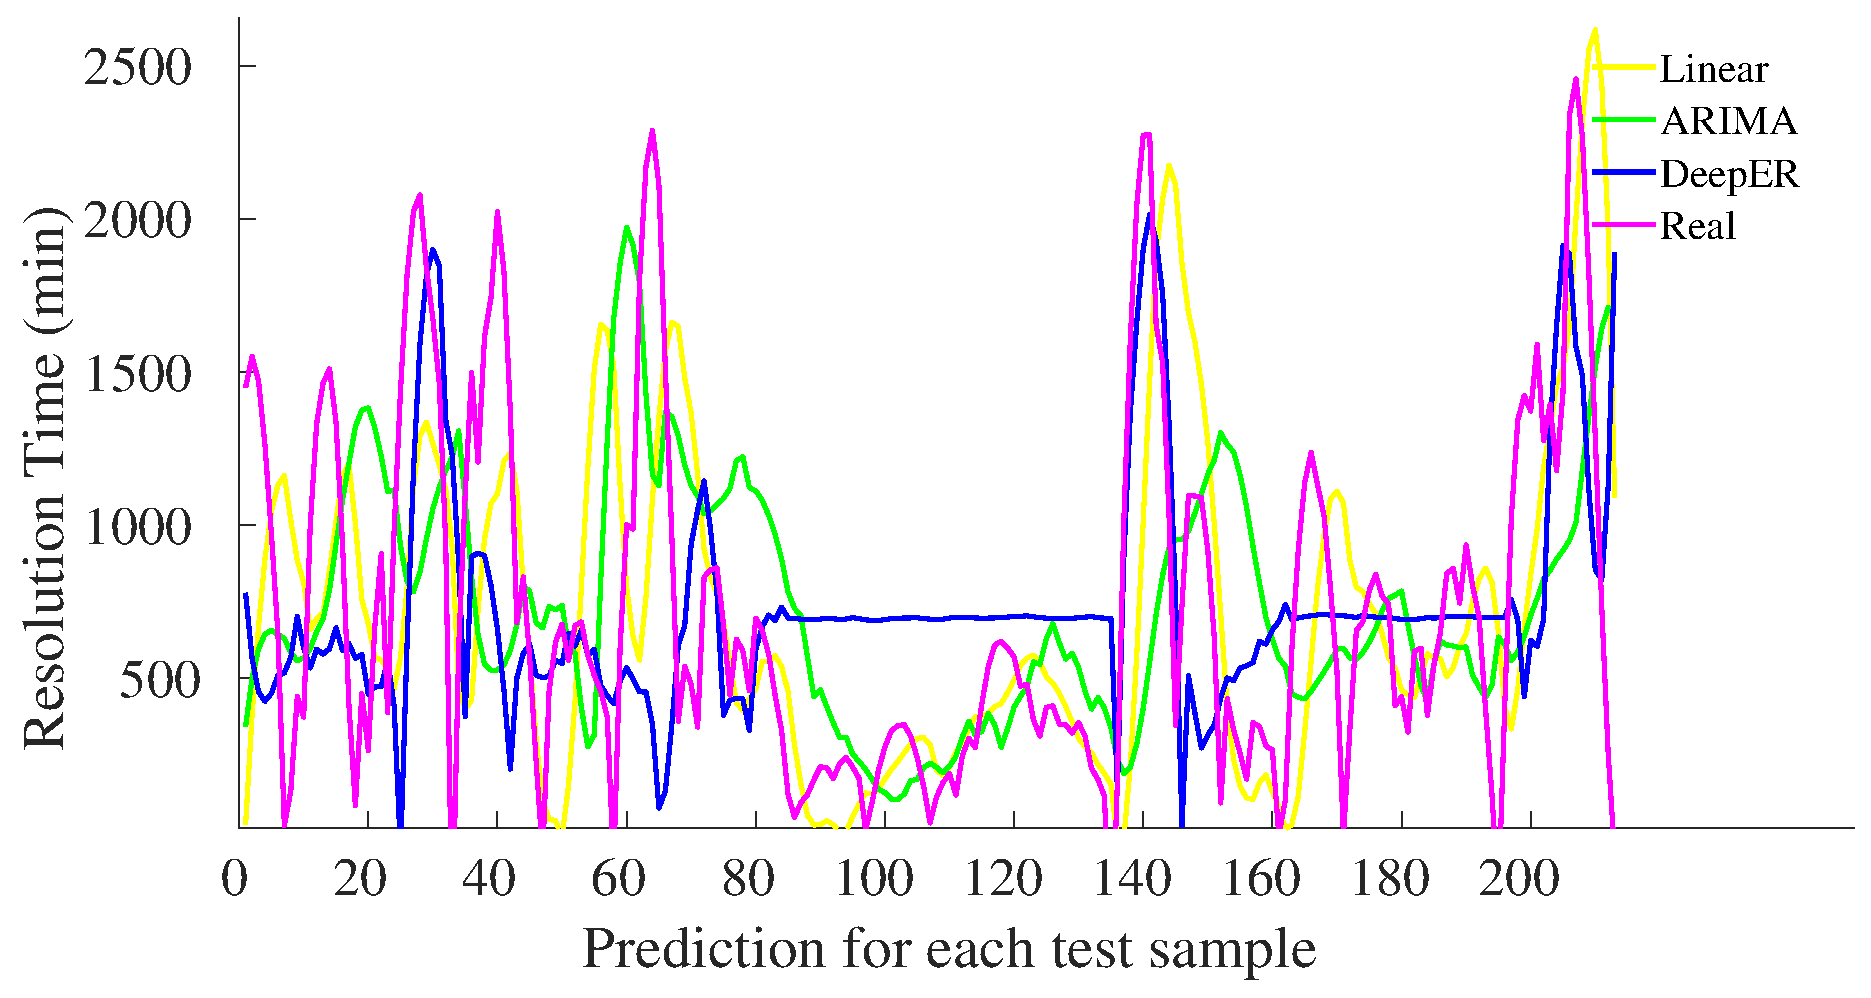
\includegraphics[width=0.9\columnwidth]{Figures/15_5/Dist/1Structural_main_7}
%       \label{5b}}
%	\caption{Real vs Predicted Fire, Law and Structural Comparison of baselines and our approach}
%  \label{fig:qualitative} 
%  \vspace{-3mm}
%\end{figure}

\begin{figure}[!ht]
  \centering
  	\label{fig:qualfire}
       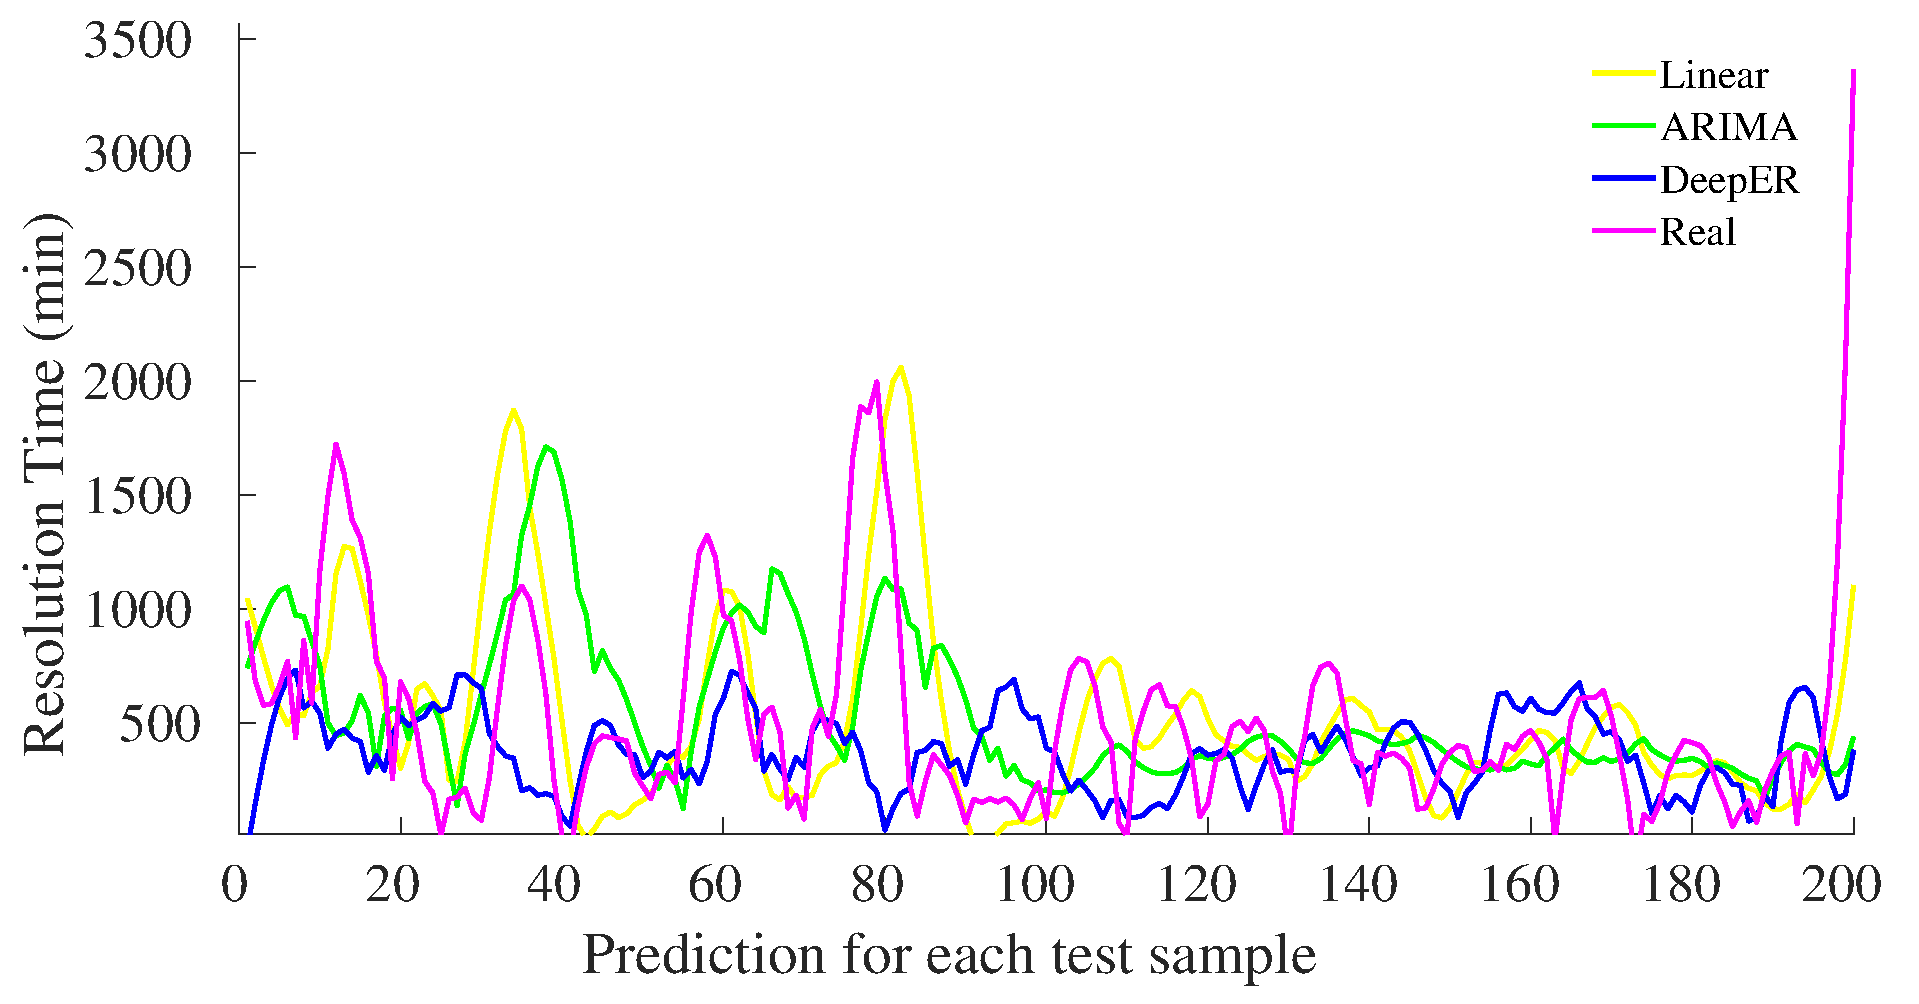
\includegraphics[scale=0.25]{Figures/15_5/Dist/1Fire_main_5}
	\caption{Fire: One step Real vs Predicted Performance}
  \label{fig:qualitative} 
  \vspace{-3mm}
\end{figure}





\subsection{Further Insights into Data Preprocessing}

As mentioned in Section \ref{Data:Preprocessing}, we ensure that the training, validation, and test data include sequences from all years of the dataset. While cross-validation is commonly used to establish the significance of the results, we design this well-crafted split of the dataset to render greater credibility to our results primarily because of the fairly limited number of data points. Additionally, as noted earlier, the dataset contains a non-trivial number of outliers and missing values.  Table \ref{table:outmiss2} shows the number and  percentage of missing and outlier points in each of the training, validation and test sets if the data is split chronologically. This uneven distribution of the outlier and missing values further necessitates a carefully constructed split to ensure that training, validation, and test sets contain a more uniform distribution of such points. We note that while the dataset is relatively small in size, each event corresponds to an emergency and therefore, it is crucial to use all available data points and generate superior predictions because such predictions are critical to improving human safety. 



\begin{table}[!ht]
\centering
\resizebox{\columnwidth}{!}{
\vspace{3mm}
\begin{tabular}{|c|c|c|c|c|}
\hline
\multicolumn{2}{|c|}{\textbf{Incident Type}}&\textbf{Training}&\textbf{Validation}&\textbf{Testing}\\
\hline
%\textbf{Incident Type}& &\textbf{Num Points}& \textbf{\% Out}& \textbf{\% Missing}\\
%\hline
\multirow{3}{*}{Fire} & Total& 1529  & 764  &764\\
&Outliers &8\% &6\%&5\%\\
&Missing &14\% &47\%&53\%\\
\hline
\multirow{3}{*}{Law} & Total& 519  & 260  &260\\
&Outliers &8\% &6\%&13\%\\
&Missing &2\% &17\%&27\%\\
\hline
\multirow{3}{*}{Structural} & Total& 754  & 377  &377\\
&Outliers &8\% &6\%&13\%\\
&Missing &2\% &17\%&27\%\\
\hline
%\multirow{3}{*}{Utility}  & Total& 942  & 471  &471\\
%&Outliers &9\% & 7\% & 6\%\\
%&Missing &2\% & 33\% & 56\%\\
%\hline
\end{tabular}
}
\caption{Statistics of Outliers and Missing values in a Chronological Split}
\label{table:outmiss2}
\vspace{-5mm}
\end{table}




\subsection{Limitations of Enriching DeepER}

We observe from Section \ref{sec:data} that each incident type consists of multiple subtypes. We attempt to perform resolution time prediction at the subtype level, but realize that because this is an emergency  events dataset, the number of data points  is not sufficient for training, validation, and testing of deep learning models for  each subtype separately. We also use these subtypes as features in DeepER, but observe that this enhanced model did not improve prediction performance. We believe that dearth of data at the subtype level is the primary reason behind it not contributing to DeepER's prediction performance.

\subsection{Practicality of DeepER}

With the increase in computational power over the last decade, deploying deep learning based systems to solve real-world problems is becoming relatively easy. As is the case with most deep learning models, DeepER requires some computational time for training. However, once trained, DeepER requires limited amount of  time to generate predictions, a desired attribute in a practical system. Additionally, as more data becomes available, DeepER can be easily retrained thus enabling it to adapt to changing situations. We anticipate DeepER to be retrained at comparatively infrequent intervals (i.e., only when significant number of new emergency events have been resolved).



%The usual split in chronological order, train, validation, test, made the percentage of invalid points (outliers and missing values) in the validation and test set at least triplicate the percentage of missing values in the training set for all the group types.  This approach lead us to poor quantitative and qualitative results. For this reason, we distritube the replacement of these invalid values fairly among training, validation and test set, as explained in section \ref{sec:data}. Other preprocessing approaches lead us to relative similar quantitative results. One of these approaches was to remove missing values. A second approach was replacing values larger than initial quantile 90 with the quantile 90 value for each incident type.
%%In this section, we add more insights to the visual analysis and support the decisions of spliting in a different way. 
%As a summary, we can say that these approaches generated flat predictions or very similar along the multi-step predicion and among instances. 
%A last approach we tried was to simplify the replacement generation with sampling randonmly from the valid points in each type. We notice that predictions still show the variations that we expected, however RMSE values increased slightly.







\section{Conclusion and Future Work}
\label{sec:conclusion}
%!TEX root = paper.tex

In this paper, we presented DeepER, a deep learning based emergency resolution time prediction system that predicts future resolution times based on past data. We performed experiments on the NYC Emergency Response Incidents data provided by NYC Open Data. We compared the performance of DeepER with ARIMA and Linear Regression using two metrics--- Root Mean Squared Error (RMSE) and Mean Absolute Error (MAE). DeepER achieved an average performance improvement of 3\% and 16\% with respect to RMSE and 10\% and 27\% with respect to MAE over ARIMA and Linear Regression, respectively. We also draw upon important learnings and insights from the data, which can be utilized for designing deep learning models for data in the emergency response domain and other related domains where the data can lack an overt predictable trend.
As part of our future work, we plan to extend this analysis to  other cities so that it gives greater validity to our results. We want to also engage with city officials so that DeepER can be adopted to aid the planning and preparation of city emergency response systems.

%we plan to continue working on a better approach for the replacement of invalid points (outliers and missing values). We would try sampling from valid points of the same year or month. In that way the replacement are closer in time. Another approach is to sample according to the subtype.
%Finally, we suggest further analysis on the sparsity of peaks in the incident types. That might be a reason why, for few incident types, we underperform compared to ARIMA. The sparsity of the peaks might be related to the availability of the models to identify flexible dynamic-length instances pattern.


%We designed a preprocessing phase according to the challenges found in the data. As almost 22\% and 8\% were missing and outlier values, we showed one way in which they can be replaced and commented about a previous more simple approach (random sampling). 

%%
%% The next two lines define the bibliography style to be used, and
%% the bibliography file.
\bibliographystyle{IEEEtran}
\bibliography{acmart}

\end{document}